%
% $Id: thesis_sample.tex 809 2015-08-27 01:44:59Z fukuyasu $
%
\documentclass[11pt]{jreport}
\usepackage{wuse_thesis}
\usepackage{indentfirst}
\usepackage[dvipdfmx]{graphicx}  % ←graphicx.styを用いてEPSを取り込む場合有効にする


% 他のパッケージ・スタイルを使う場合には適宜追加
\usepackage{amsmath,amssymb,bm}  % 数式のパッケージ
\usepackage{subcaption}
\usepackage{enumerate} % 箇条書き
\usepackage{lscape} % 横向き
\usepackage{comment}
\usepackage{tipa} % IPS symbols essential for name of GESI/GEDI
\usepackage{cite}
\usepackage{otf}  % 宮﨑の漢字を入れるために必要  
                  % https://osksn2.hep.sci.osaka-u.ac.jp/~taku/osx/old/gaiji.html

% \usepackage[dvipdfmx]{color}
\usepackage{threeparttable}
\usepackage{here}
% \usepackage{url}	% \url{}コマンド用。URLを表示する際に便利

% Table
\usepackage{booktabs, multirow} % for borders and merged ranges
\usepackage{soul} % for underlines
\usepackage[table]{xcolor} % for cell colors
\usepackage{changepage,threeparttable} % for wide tables

\usepackage{otf} % ローマ数字
\usepackage{url} % 参考文献のURL

% \usepackage[dvipdfmx]{graphicx}

% \makeatletter
% \newcommand{\figcaption}[1]{\def\@captype{figure}\caption{#1}}
% \newcommand{\tblcaption}[1]{\def\@captype{table}\caption{#1}}
% \makeatother

% \usepackage{here}
% \usepackage{comment}
% \usepackage{caption}			
% \usepackage{latexsym}
% \usepackage{cite}
% \usepackage{pifont}

% \usepackage[dvipdfmx]{graphicx}
% \usepackage{subfig}
% \usepackage[dvipdfmx]{color}
% \usepackage{unicode-math}
% \usepackage[ipaex]{pxchfon}

% \usepackage{latexsym}
% \usepackage{amssymb}

% \usepackage{amssymb}
% \usepackage{amsmath}

% \usepackage[ipaex]{pxchfon}
% \usepackage{array, booktabs, multirow}
% \usepackage{wrapfig}
% \usepackage{subfig}
% \usepackage[dvipdfmx]{color}
% \newcommand{\argmax}{\mathop{\rm argmax}\limits}
% \newcommand{\argmin}{\mathop{\rm argmin}\limits}

% % Add, YA, January 2023
% \usepackage{tipa} %IPS symbols essential for name of GESI/GEDI
% \usepackage{lscape} % 横幅の大きい表を回転


%%%%%%%%%%%%%%%%%%%%%%%%%%%%%%%%%%%%%%%%%%%%%%%%%%%%%%%%%%%%%%%%%%%%%%%%

%%
%% 主に表紙を作成するための情報
%%

%%  タイトル(修論の場合は英語表記も指定)
\title{高齢者における\\感情音声の弁別特性についての研究}
\etitle{A Study of Discrimination Characteristics of Emotional Speech in Older Adults}

%%  著者名(修論の場合は英語表記も指定)
\author{花谷 幸歩}
\eauthor{Yukiho Hanatani}

%% 卒業論文・修士論文(以下のどちらかを選択)
%\bachelar	% 卒業論文(4年生用)
\master  	% 修士論文(M2用)

%%  学科・クラスタ
%\department{情報通信システム}
\department{システム知能}
%\department{デザイン科学}

%%  学生番号
\studentid{S2320107}

%%  卒業年度
\gyear{2024}		% 提出年が2015年なら,2014年度

%%  論文提出日
\date{2025年2月}	% 修士の場合は月(2015年2月)までとし,英語表記も指定
\edate{February 2025}	% 修士の場合,こちら(英語表記)も有効化

%%%%%%%%%%%%%%%%%%%%%%%%%%%%%%%%%%%%%%%%%%%%%%%%%%%%%%%%%%%%%%%%%%%%%%%%

\begin{document}

\maketitle

%%
%%  概要
%%


\begin{abstract}
\textcolor{red}{【--------未編集--------】超高齢社会を迎えた現在、高齢難聴者個人ごとに対応した音声・聴覚支援機材の開発が急務である。そこでは、音声強調処理/雑音抑圧処理が必須の技術となっている。この開発のためには、聴取者による処理音声の主観評価実験と、その結果を精度良く予測する客観評価指標が不可欠である。音声強調処理の評価基準として広く利用されているSTOIをはじめ、これまで数多くの客観評価指標が提案されてきた。しかし、これらの手法は健聴者に対応したもので、難聴者個人の特性を適切に反映できないものがほとんどである。}

そこで本論文では、高齢難聴者の音声了解度予測を目指した新たな客観評価指標Gammachirp Envelope Similarity Index (GESI)を提案した。これは、基準音声と評価音声を、ガンマチャープ聴覚フィルタバンク(GCFB)と変調周波数フィルタバンク(MFB)の組み合わせで分析し、特徴量間の拡張コサイン類似度を計算して統合した指標である。
基準音声と評価音声の間の音圧レベル差や、聴取環境における閾値上レベルを適切に反映できる。

このGESIが3種類の主観評価実験結果を精度良く予測できるかを、従来手法と対比して評価した。
まず、模擬難聴音声システムWHISで高齢難聴者の聞こえにくさを模擬した音声に対する健聴者の主観評価結果を用いた。
WHISを用いたのは、実際の高齢難聴者実験で起こりうる機能低下の度合いや要因による結果のばらつきを抑え、聴覚末梢系の機能低下だけを評価するためである。これは、高齢難聴者個人ごとの予測の基礎になる。
従来手法STOIやその派生型は、内部指標計算時に行われる音圧正規化処理のため全く予測できなかった。
補聴器処理の評価のために提案されたHASPIは、聴取環境による了解度の変化を予測できなかった。
一方、GESIは話者性別や聴取環境(防音室/クラウドソーシングによる遠隔)にかかわらず、個人別に精度良く予測できた。
次に、模擬難聴処理に対して補聴器信号処理(処方式)を施した場合の主観評価了解度を予測した。GESIは、処方式による了解度の違いをHASPIよりも概ねよく予測できた。
これにより、補聴器装用時の音声了解度予測にも使用できる可能性が示唆された。
最後に、マルチチャンネルと理想的なシングルチャンネルの音声強調処理に対する健聴者の音声了解度を予測できるか検証した。
その結果、GESIは従来手法であるSTOIやその派生型と同程度の精度で予測できることがわかった。
これにより、難聴条件ばかりでなく、音声強調処理の開発全般にも利用できることが示された。

以上のことから、従来手法や補聴器信号処理の評価指標に取って代わる客観評価指標として有効であることが示された。


\end{abstract}

%%  目次
\tableofcontents

%%  図目次 (図目次をいれたければ以下のコメントをはずす)
%\listoffigures

%%  表目次 (表目次をいれたければ以下のコメントをはずす)
%\listoftables

\newpage
\pagenumbering{arabic}	% 以降のページ番号を算用数字に

%%%%%%%%%%%%%%%%%%%%%%%%%%%%%%%%%%%%%%%%%%%%%%%%%%%%%%%%%%%%%%%%%%%%%%%%

%%
%%  本文はここから
%%
%%%%%%%%%%%%%%%%%%%%%%%%%%%%%%%%%%%%%%%%%%%%%%%%%%%%%%%%%%%%%%%%%%%%%%%%


%%%%%%%%%%%%%%%%%%%%%%%%%%%%%%%%%%%%%%%%%%%%%%%%%%%%%%%%%%%%%%%%%%%%%%%%%%%%%%%%%%
%%%%%%%%%%%%%%%%%%%%%%%%%%%%%%%%%%%%%%%%%%%%%%%%%%%%%%%%%%%%%%%%%%%%%%%%%%%%%%%%%%
\chapter{はじめに}
\label{chap:Intro}
%%%%%%%%%%%%%%%%%%%%%%%%%%%%%%%%%%%%%%%%%%%%%%%%%%%%%%%%%%%%%%%%%%%%%%%%%%%%%%%%%%
%%%%%%%%%%%%%%%%%%%%%%%%%%%%%%%%%%%%%%%%%%%%%%%%%%%%%%%%%%%%%%%%%%%%%%%%%%%%%%%%%%


%%%%%%%%%%%%%%%%%%%%%%%%%%%%%%%%%%%%%%%%%%%%%%%%%%%%%%%%%%%%%%%%%%%%%%%%
\section{研究背景}
%%%%%%%%%%%%%%%%%%%%%%%%%%%%%%%%%%%%%%%%%%%%%%%%%%%%%%%%%%%%%%%%%%%%%%%%
\label{sec:研究背景}
超高齢社会となった日本では、加齢性難聴者の増加が懸念されている。
聴力低下は、音声による対人コミュニケーションを妨げ、生活の質(QOL)の低下を招く。
また、認知症リスクを高める最大要因であることがLancet委員会により報告されている\cite{livingston2020dementia}。
高齢者との円滑なコミュニケーションのためには、音声の言語情報ばかりではなく、感情を含む非言語情報も重要である。
特に感情(情動)は、言語情報と異なり曖昧で、高齢者にどの程度意図した通りに伝達できるかの特性もまだよくわかっていない。
これまでに、加齢により感情認識精度が低下することが報告されている\cite{paulmann2008aging,ben2019age,amorim2021changes}。
特に否定的な感情に関して低下するという報告もある\cite{mill2009age}。
また、従来からの補聴器で音声了解度の改善は行うことができるが、感情伝達特性の向上には貢献しないことが報告されている\cite{goy2018hearing}。
感情知覚機能の低下の要因は、聴覚末梢系の機能低下による聴力レベルによるものだけとは考えられてはいない。
しかしながら、明確にそのことを示す実験データは存在しないようである。
また、末梢系から認知系のどの部位の機能低下によるものかも解明されていない。
そこで、まずは聴覚末梢系の機能低下だけが、感情知覚にどの程度影響するかの調査を試みた。
若年健聴者に模擬難聴処理を行った音声を聴かせ、通常音声を聴いた場合との感情知覚の相違を実験的に検討した。
さらに、高齢者の感情知覚特性を、同じ通常音声を用いて同じ手順で測定した。
若年健聴者との相違から知覚特性の情報を得ることを目指した。

% SciRep
% 難聴(HL)を抱える高齢者の数は多くの国で増加している。
%  HLによる対人コミュニケーションの低下は、生活の質(QOL)を低下させるだけでなく、認知症の極めて高い危険因子であることが示されている1。
% 音声は、言語的内容と、話し手の特徴や感情を含む副言語的情報の両方を伝えます。
% 従来の補聴器は、主に音声の明瞭度を向上させるように設計されており、感情的なコミュニケーションを改善するものではない。
%  音声の感情認識2-5とその加齢効果6-14に関する研究は数多く行われており、加齢とともに感情認識・識別能力が低下することが報告されている。
% 補聴器は明瞭度を向上させるにもかかわらず、感情認識を向上させないことが確認されている9。
% 加齢は、蝸牛から中枢神経系に至る聴覚プロセスに影響を及ぼす。
% 一つの研究課題は、加齢に関連した末梢の聴覚障害が感情認知にどの程度影響するのか、また異なる段階でどのような過程が関与するのかということである。
% もう一つの疑問は、感情知覚をサポートする新しい補聴器を開発できるかどうかということである。
% 感情の低下が、認知のみによるのではなく、主に音声の特徴や声の表情の聴覚的表現の劣化によって引き起こされるのであれば、新しい強化アルゴリズムを開発することも可能であろう。

% 【copied 2022】世界に先駆けて超高齢化社会へ突入した日本では,今後も老人性難聴者が増加することは間違いない.
% 聴力低下による対人コミュニケーションの減少は,生活の質(Quality of life:QOL)を下げることに繋がる\cite{lancet}.
% また,老人性難聴は認知症の極めて高い要因であることが指摘されている\cite{AgeHL}.一般的に,難聴の対処には補聴器が挙げられる.
% その一方で,補聴器は難聴者の15\%ほどしか利用されておらず\cite{JPTrack},万人に有効な手立てとはなっていない.今までの補聴器は,
% 主に聞き取りやすさ(音声了解度)の改善だけを目的とされてきた.しかし,難聴者との円滑なコミュニケーションのためには音声了解度だけでなく,
% 感情の伝わりやすさ(感情伝達特性)についても考慮する必要があると考える.
% 老人性難聴者に話しかける際には「大きな声でゆっくりと話す」ことがよいとされている.ところが,これを表層的に捉えて単に大きな声で話しかけると,
% 「叱られている」と高齢者に勘違いされることがある.聴力レベルや言語情報処理から見た従来の理論においては正しいとされる方法であるにもかかわらず,
% 「感情」が伝わらないということは,感情伝達についての知見が不十分な証拠である.

% 本研究の将来的な目標は,老人性難聴者を含む他者への感情伝達特性を解明し,定式化することである.これにより,
% 補聴器の開発や超高齢社会における対人コミュニケーションの改善に繋がると考える.


%%%%%%%%%%%%%%%%%%%%%%%%%%%%%%
\section{研究目的}
%%%%%%%%%%%%%%%%%%%%%%%%%%%%%%
\label{sec:研究目的}

本研究の目的は、高齢者の感情知覚特性について調査することである。
将来的には、その特性を定式化し、補聴器の開発や高齢者との円滑なコミュニケーションに貢献することを目標としている。

本研究では、2つの実験を実施する。
1つ目は、若年健聴者実験である。
若年健聴者に難聴者の聞こえを体験させる「模擬難聴システムWHIS」(以下WHIS)を用いた聴取実験を行い、模擬難聴が感情知覚に与える影響を調査する。
通常音声を聞いた場合と、模擬難聴処理した音声を聞いた場合の結果に差異があるかどうかを確かめる。
WHISを用いて実験を行う理由は以下である。
加齢性難聴の原因は様々であり、聴覚末梢系の機能低下によるものか、中枢系・認知系の機能低下によるものかの切り分けが困難である。
どの原因がどの程度感情知覚に影響するのかを段階的に調査するために、まずは模擬難聴処理で聴覚末梢系の機能低下だけを模擬することにした。
したがって、WHISで処理した音声を聞いた若年健聴者を「模擬難聴者」として実験を行う(詳しくは第\ref{chap:ExpAngHapSad}章で説明する)。

2つ目は、高齢者実験である。
若年健聴者実験と同じ通常音声・手順で実験的に測定を行う。
若年健聴者結果と比較することで、聴覚末梢系の機能低下による感情知覚への影響があるかどうかを検証する。
また、聴覚末梢系の機能低下以外の要因も調査できると考え、実施することにした。

これらの実験から、若年健聴者が通常音声を聞いた場合・若年健聴者が模擬難聴処理音声を聞いた場合・高齢者が通常音声を聞いた場合の
感情音声の弁別精度を比較する。
以上の3条件の違いから高齢者の感情知覚特性について新たな知見を得ることを目的に実験を行った。


%SciRep
% 第一の研究課題に答えるためには、高齢者では変動が大きい聴覚経路や認知の要因を除外し、末梢HLのみがパーフォーマンスに及ぼす影響を特定する必要もある。
% この目的のために、健聴者(NH)にHL体験を提供するHLシミュレータを実験に使用することができる。
% HL模擬音を使った怒りの知覚に関する最近の実験がある14。
% 動機は似ているが、彼らの実験は基本的に感情識別課題であった。

%本研究では、音声モーフィングツールとHLシミュレータWHIS24を組み合わせて、感情ペア間の感情弁別実験を行った。
% 若年NH(YNH)参加者が通常の音を聞いた場合、同じYNH参加者がHL模擬音を聞いた場合、高齢参加者が同じ通常の音を聞いた場合の識別性能を比較した。
% これら3つの条件の違いから、高齢者の感情知覚の特徴について新たな知見が得られるかもしれない。

% 【copied 2022】本研究は,健聴者に難聴者の聞こえを体験させる「模擬難聴システムWHIS」(以下WHIS)を用いた聴取実験を行い,
% 模擬難聴が感情知覚に与える影響を調査することを目的とする.将来的な目標は,老人性難聴における感情伝達特性の解明と定式化である.


% WHISを用いて実験を行う理由は以下の2つである.第一に,実際の老人性難聴者を対象とした場合,難聴の原因が末梢系の機能低下によるものか,
% 認知機能の低下によるものかの切り分けが困難であり,個人ごとのばらつきも大きい.第二に,新型コロナウイルスの影響もあり高齢者を対象とした実験は難しい.
% このような理由から,WHISで処理した音声を聞いた健聴者を「模擬難聴者」として実験を行う(詳しくは,第\ref{sec:感情知覚実験}章で説明する).

% 本研究では,同一被験者で健聴状態と模擬難聴状態で聴取実験を行い,感情判断の差異をもとに模擬難聴が感情知覚に及ぼす影響について調査する.


%%%%%%%%%%%%%
\section{本論文の構成}
%%%%%%%%%%%%%
\label{sec:本論文の構成}
本論文は、本章を含めて5章で構成されている。
第1章では、本研究の背景と目的について示した。
第2章では、聴覚に関する基本的な知識と、音声と感情知覚に関する従来研究について説明する。
第3章では、怒り・悲しみ・喜び間の弁別実験について、詳細な手続きを述べた上で、結果についてまとめる。
第4章では、落着きと怒り・悲しみ・喜び間の弁別実験について、手続きと結果についてまとめる。
また、第3章の怒り・悲しみ・喜び実験の結果と比較検討する。
最後に、第5章で本研究について総括する。

% 【copied 2022】本論文は,本章を含め6章で構成されている.第1章では,本研究の背景と目的について示した.第2章では,聴覚に関する基本的な知識と,音声と感情知覚に
% 関する知識,先行研究について説明する.第3章では,本実験の詳細な手続きを述べる.第4章では実験結果と統計的分析を行なった結果を示し,第5章で考察を述べる.
% 最後に,第6章にて本研究についてまとめる.



%%%%%%%%%%%%%%%%%%%%%%%%%%%%%%%%%%%%%%%%%%%%%%%
%%%%%   聴覚に関する背景知識と感情音声知覚  %%%%%
%%%%%%%%%%%%%%%%%%%%%%%%%%%%%%%%%%%%%%%%%%%%%%%
\newpage
\chapter{聴覚に関する背景知識と感情音声知覚}
\label{chap:RelatedResearch}

この章では
まず、主に文献\cite{ogushi2019Book, furukawa2021chokaku}を引用して、聴覚に関する基本的な知識や聴覚系における情報分析機能とそのモデル化について述べる。
次に、難聴の種類や高齢者の聴覚特性、模擬難聴処理について述べる。
\textcolor{red}{そして、心理学における感情分類について説明し、これまでに行われてきた感情音声認識実験とその課題について議論する。}


%--------------
\section{聴覚系の概要}
\label{sec:Auditory}
%--------------
%参考 山本さん修論 
ヒトの耳は、外耳、中耳、内耳の3つの部分から構成され、聴神経を経て脳へとつながっている。
その様子を図\ref{fig:Hearingsystem}に示す。
耳に到来した音は、耳介の複雑な構造による反射音・直接音の干渉のため、音のスペクトルに変化が生じる。
このスペクトル変化は、音源の空間的位置に依存し、聴空間知覚、特にどの方向から音が聞こえているかという上下・前後方向の音源定位の知覚を可能にする。
外耳道を経た音は鼓膜を振動させ、ツチ骨、キヌタ骨、アブミ骨と呼ばれる3つの耳小骨の連鎖を通じて、内耳へと伝えられる。
内耳では、主に周波数分析が行われ、数10Hzから20kHzの音が各周波数に対応し、聴神経発火に変換される。
左右の内耳の聴神経から発せられた信号は、一部交差しながら数カ所の中継点を経て、最終的に大脳皮質に達する。
音の音色などの知覚は、大脳皮質の聴覚野によって行われる。

% ---------------------------------------
\begin{figure}[htbp]
    \vspace{40pt}
    \centering
    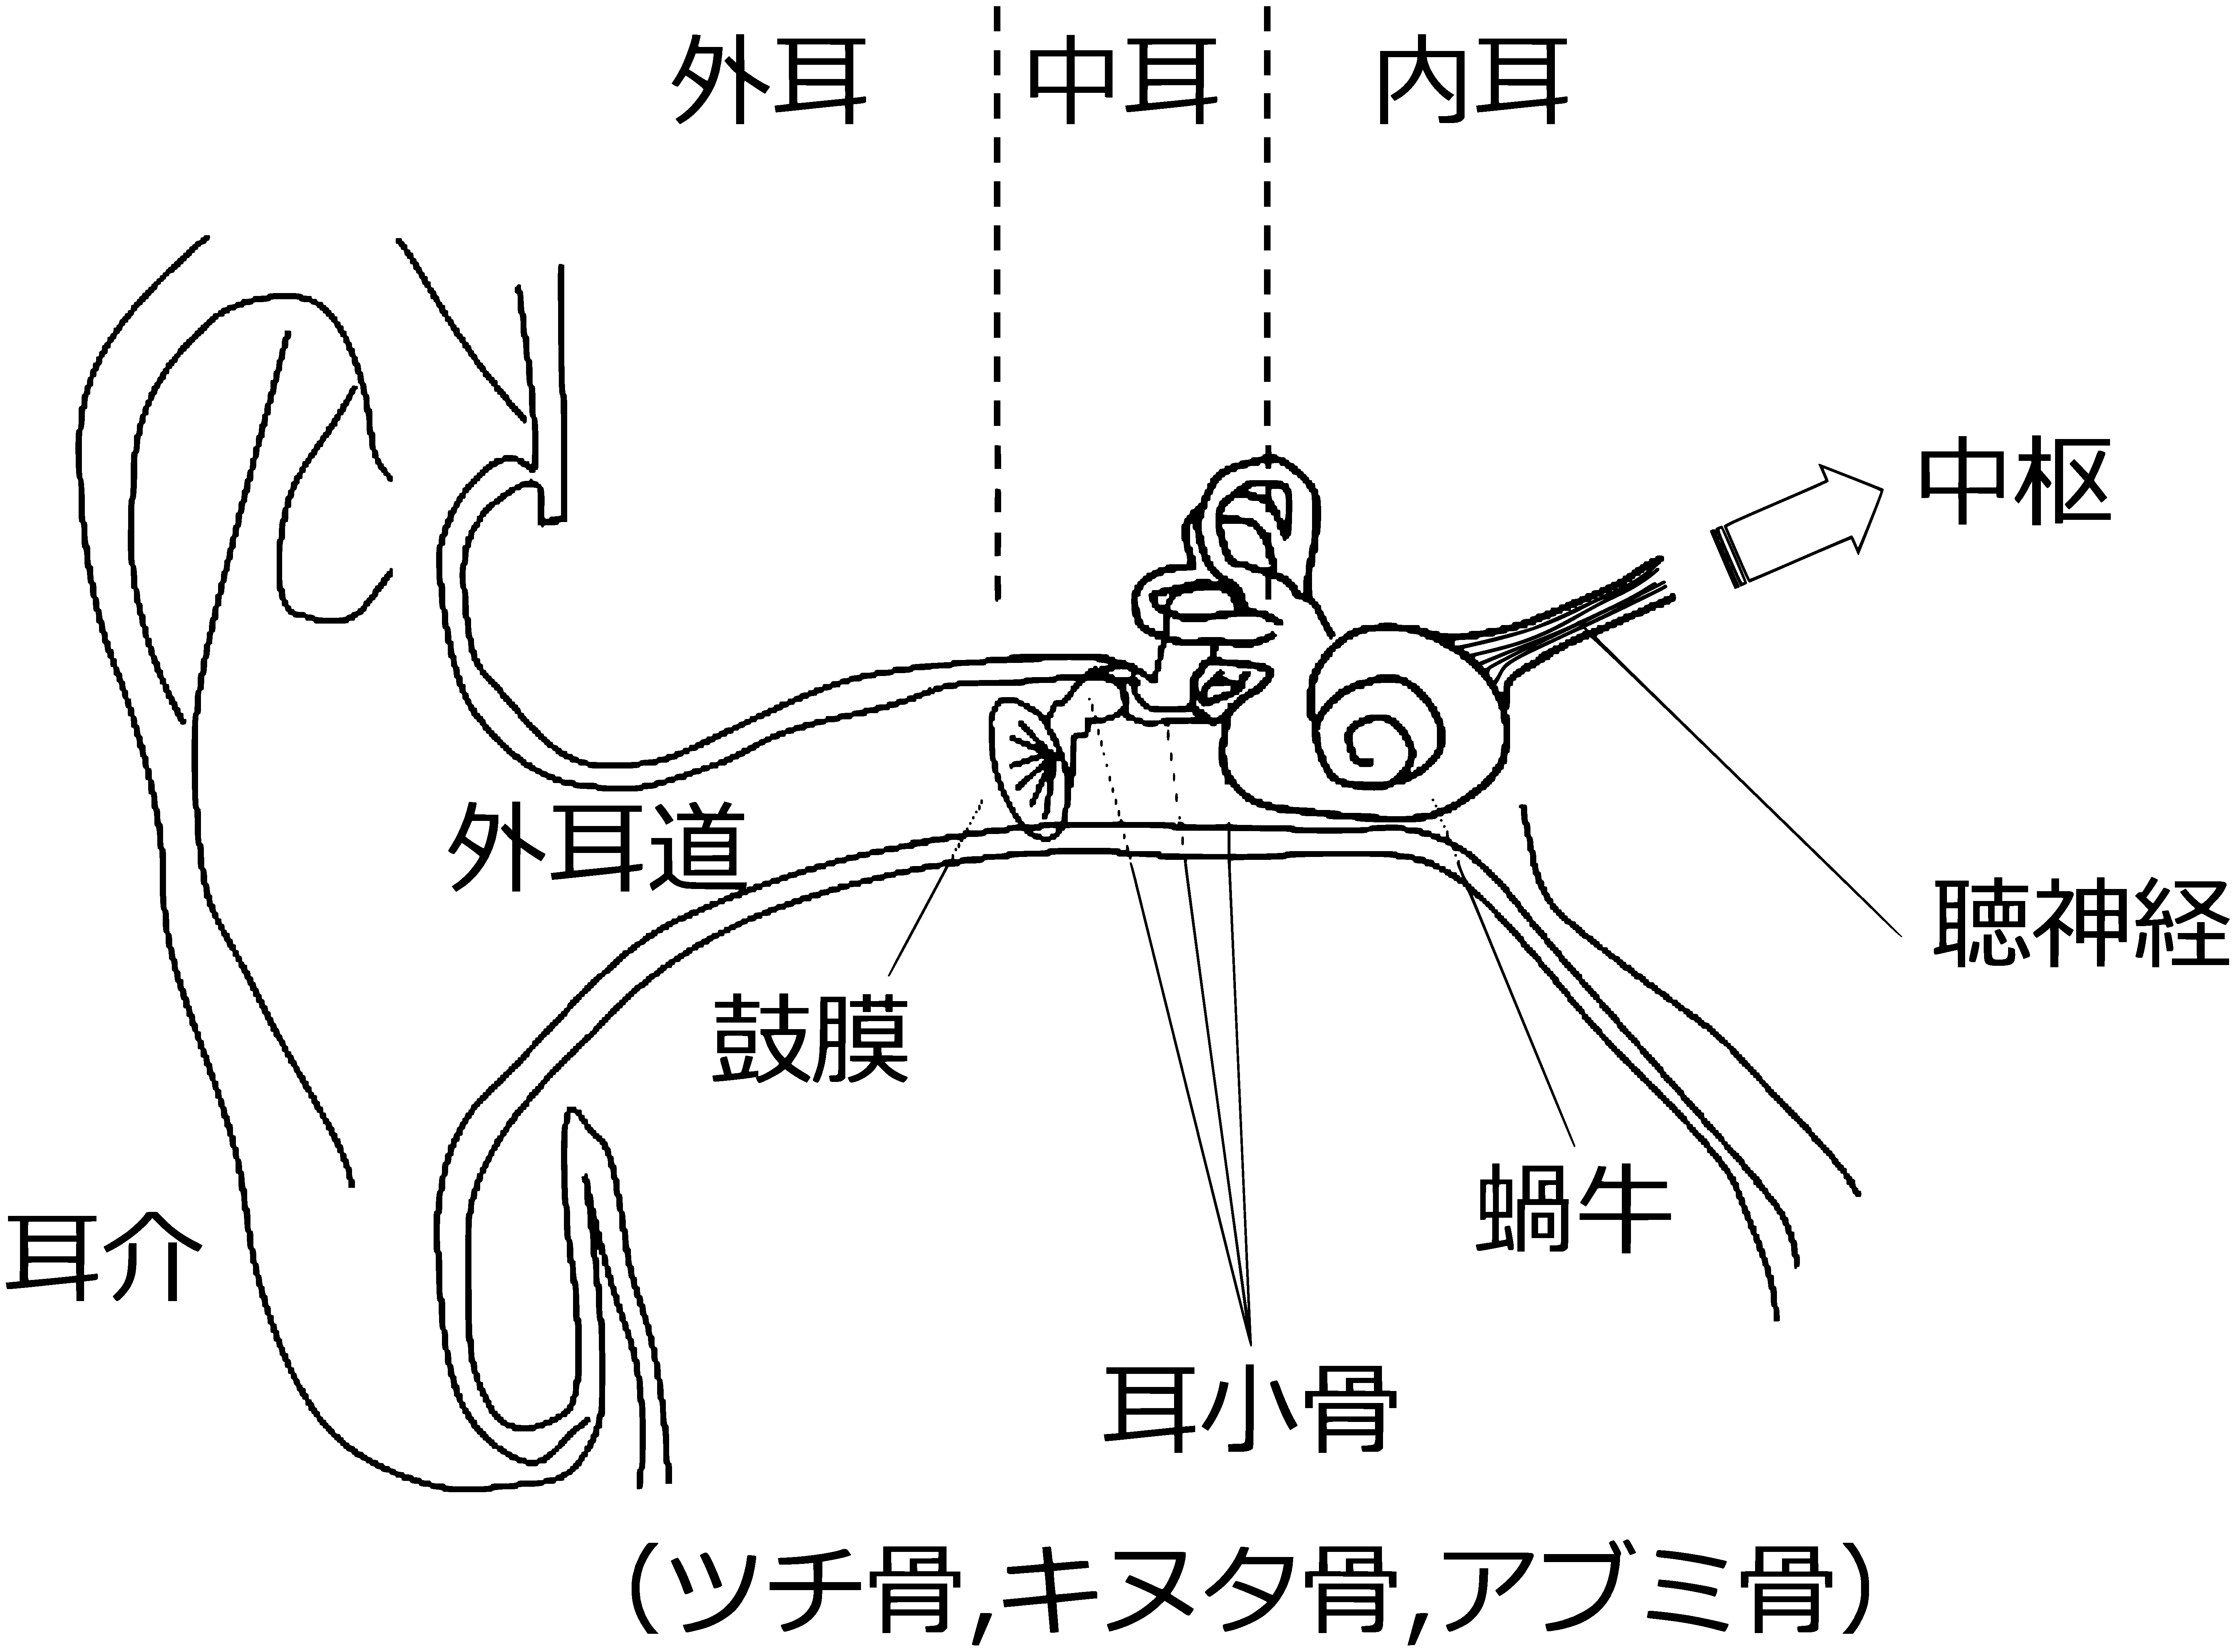
\includegraphics[width=0.6\hsize]{Figure/RelatedResearch/furukawa2017auditory.eps}
    \caption{聴覚末梢系の概観。文献\cite{furukawa2017chokaku}の図1より引用。}
    \label{fig:Hearingsystem}
\end{figure}
% --------------------------------------------


% ==============================
\section{周波数分析機能}
% \label{sec:peripheral}
% ==============================

% ------------------------------
\subsection{聴覚フィルタ}
% \label{sec:auditory filter}
% ------------------------------
前節で述べたように、蝸牛に到達した音は、基底膜が機械的に振動することで周波数分析された後に聴神経発火へ変換される。
この基底膜振動に由来する周波数分析あるいは周波数選択性を、心理物理学において聴覚フィルタ(auditory filter)と呼ぶ。

基底膜の機械振動が最大となる場所は、入力された音の周波数によって変化する。
この様子は、信号処理の観点から、中心周波数と帯域幅が異なる多数の聴覚フィルタが並んでいると考えられ、
このフィルタ群全体を聴覚フィルタバンク(auditory filter bank)と呼ぶ。
蝸牛頂側には低周波数域に対応する聴覚フィルタ、耳小骨側では高い周波数に対応する聴覚フィルタが並んでいる。

% ---------------------------------------
\begin{figure}[h]
  \vspace{20pt}
  \centering
  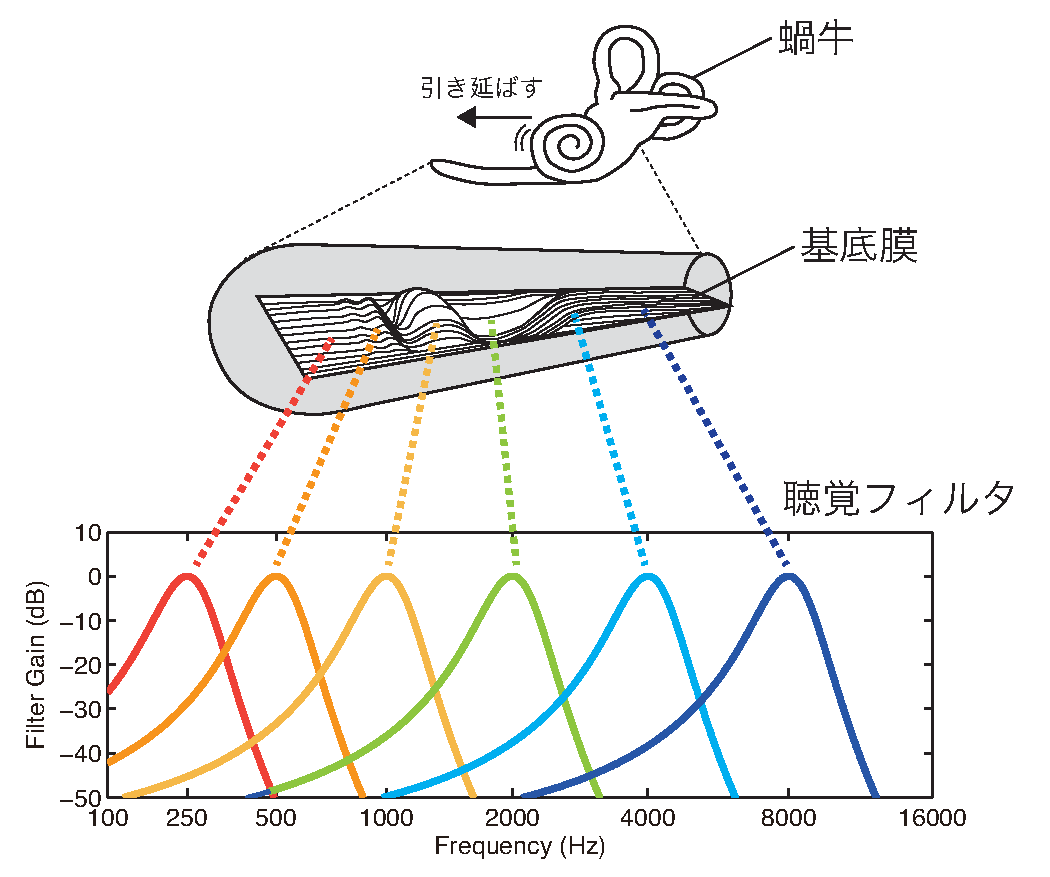
\includegraphics[width=0.6\hsize]{Figure/RelatedResearch/KiteimakuAudFilter.eps}
  \caption{聴覚フィルタの模式図。蝸牛を引き延ばした図(中段)では、基底膜の振動の様子を表している。
            入力音の周波数によって基底膜上の振動する場所が異なる。このような内耳での周波数分析は、
            聴覚フィルタ(下段)が並んでいる形で定式化できる。文献\cite{higashiyama2020WHIS}の図1.6より引用。}
  \label{fig:BasilarMembrane}
\end{figure}
% --------------------------------------------

% ------------------------------
\subsubsection{振幅周波数特性}
% ------------------------------
図\ref{fig:Basic_FilterBank}に6つの中心周波数をもつ聴覚フィルタの振幅周波数特性の例を示す。
横軸は周波数、縦軸はフィルタの利得である。
心理物理学では、このような振幅周波数特性の2乗のパワースペクトルのことをフィルタ形状と呼ぶ。
% ただし横軸は、対数周波数尺度に近い非線形周波数軸(後述の$\mathrm{ERB_{N}}$番号軸)となっている。
図\ref{fig:Basic_FilterBank}より入力された音圧が一定の場合、聴覚フィルタは中心周波数に関わらず同じような形状をもつことがわかる。
また、その周波数特性は中心周波数に対して非対称である。
さらに、外界の音圧や音環境によって変化する非線形フィルタとなっている。

聴覚フィルタの特性は個人ごとに異なり、特に高齢者や難聴者の場合は標準的な特性から大きくばらつく。
そのため、個人の特性に合わせたモデル化が必要とされている。

% ------------------------------
\subsubsection{聴覚フィルタの帯域幅}
% ------------------------------
ここで、健聴者の聴覚フィルタの中心周波数$F$Hzと帯域幅は、
おおよそ以下の関係であることが心理物理学測定から知られている\cite{moore2013introduction}。

\begin{equation}
	\mathrm{ERB_N} = 24.7 \times\bigl(\frac{4.37F}{1000} + 1\bigr)
    \label{eq:ERB}
\end{equation}

等価矩形帯域幅(equivalent rectangular bandwidth; $\mathrm{ERB_N}$)とは、
図\ref{fig:ERB}のようにある中心周波数$F$Hzの聴覚フィルタのパワースペクトル上での面積を、
聴覚フィルタの最大利得と等しい高さをもつ長方形(矩形)で表現した場合の帯域幅(底辺)である。
この等価矩形帯域幅自体は、任意のフィルタ形状で計算することができる。
この中心周波数によって変わる帯域幅のフィルタが、同一形状で等間隔に並ぶように$\mathrm{ERB_N}$番号($\mathrm{ERB_N}$ number)が定義されている(単位: Cam)。

\begin{equation}
    \mathrm{ERB_N \ number} = 21.4 \log_{10} \bigl(\frac{4.37F}{1000} + 1\bigr)
\end{equation}

% ---------------------------------------
\begin{figure}[h]
    % ---------------------------------------
    \begin{minipage}[c]{0.45\hsize}
    \vspace{50pt}
    \centering
    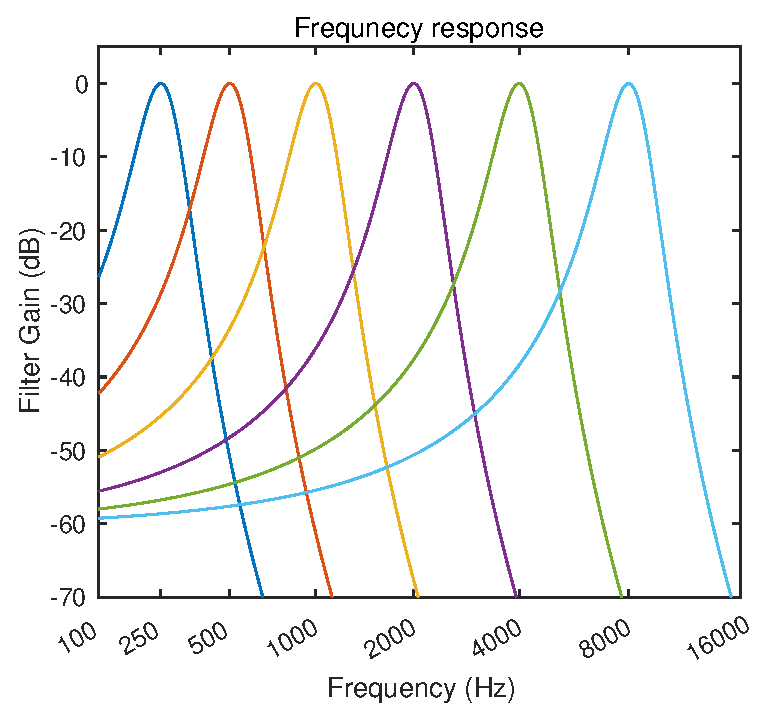
\includegraphics[width=\hsize]{Figure/RelatedResearch/DemoAF_Basic_FilterBank.eps}
    \caption{聴覚フィルタの周波数特性の例。一定音圧の場合で、中心周波数が250, 500, 1000, 2000, 4000, 8000Hzの6種類の聴覚フィルタを示す。文献\cite{irino2010hajimete}の図1より引用。}
    \label{fig:Basic_FilterBank}
    \end{minipage}
    % ---------------------------------------
    \hspace{0.1\hsize}
    \begin{minipage}[c]{0.45\hsize}
    \vspace{50pt}
    \centering
    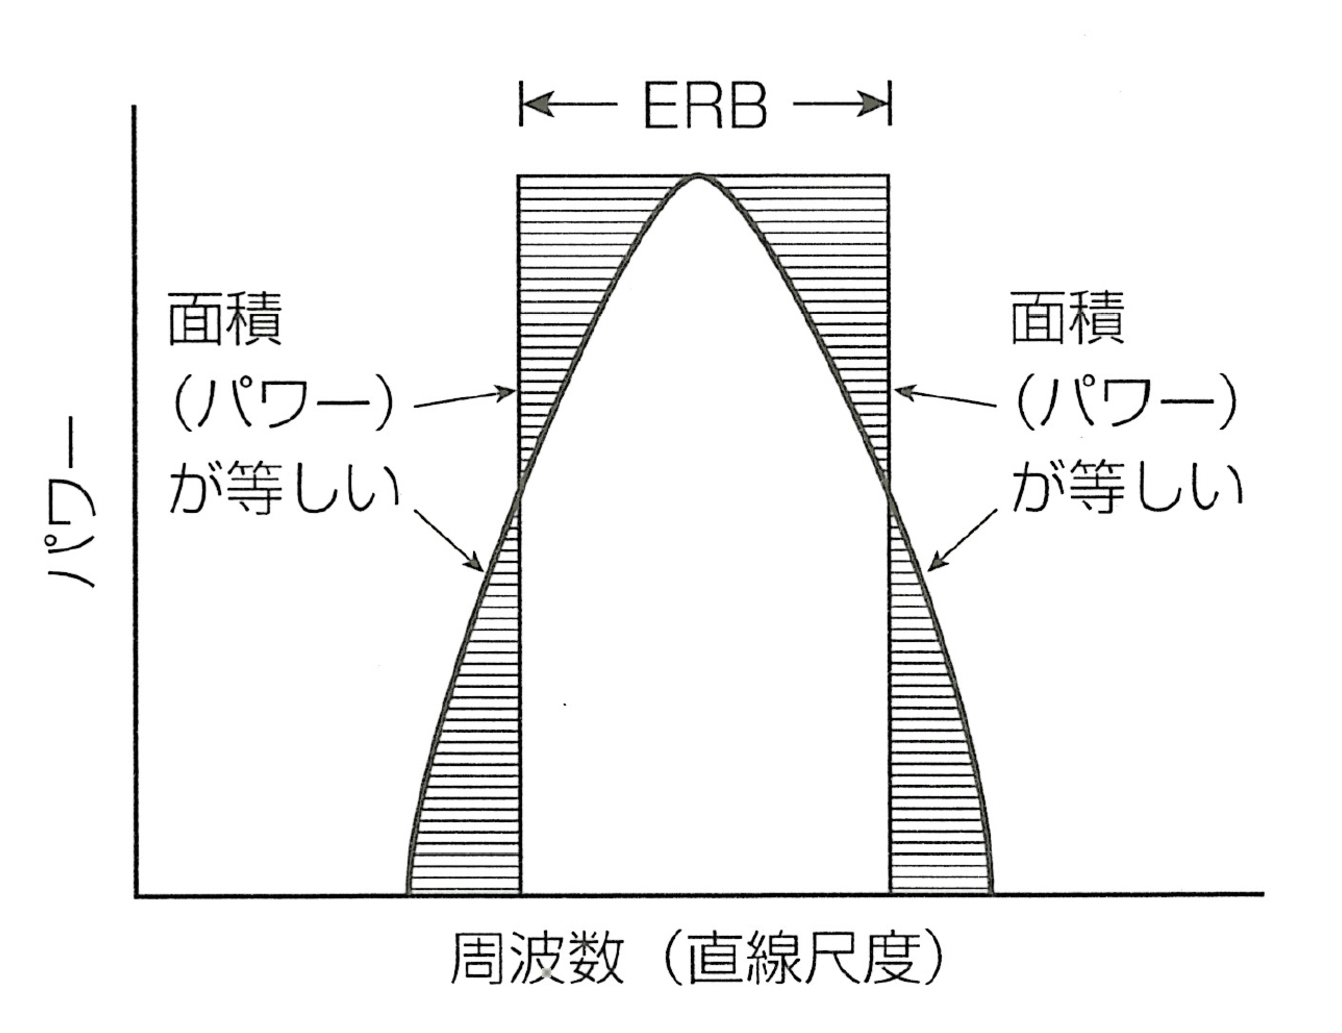
\includegraphics[width=1.08\hsize]{Figure/RelatedResearch/Ogushi2019ERB.eps}
    \caption{等価矩形帯域幅(ERB)。曲線はある中心周波数の聴覚フィルタを示す。文献\cite{ogushi2019Book}の図4-15より引用。}
    \label{fig:ERB}
    \end{minipage}
\end{figure}
% --------------------------------------------


\newpage
% ------------------------------
\subsection{音圧依存性}
\label{sec:FilterLevelDepend}
% ------------------------------
実際の聴覚フィルタは、外界の音環境や音圧に依存して、その形状や利得が変化する非線形の時変フィルタである。
音圧に対するフィルタ形状や利得変化の例を図\ref{fig:Basic_FilterLevelDepend}に示す。
入力音の音圧が30dBのとき、中心周波数における利得は最も大きく、音圧が上昇するとともに利得が減少することがわかる。
さらに、フィルタの帯域幅も音圧上昇と共にやや広くなる傾向があることもわかる。
    
% ------------------------------
\subsection{圧縮特性}
\label{sec:IOfunc}
% ------------------------------
図\ref{fig:Basic_IOfunc}は、図\ref{fig:Basic_FilterLevelDepend}で示した聴覚フィルタの特性(音圧依存性)から計算される、
フィルタの入力音圧と出力音圧の関係を示すグラフである。
破線で示された増加率が1\,dB/\,dB(1:1)の線形関係を表している。
実線で表された健聴者の聴覚フィルタの入出力特性は、破線に比べて緩やかな傾きであり、中程度の音圧域で約0.2$\sim$0.3\,dB/\,dBの増加率になると推定されている。
このような、入力音圧が小さい場合利得が大きく、入力音圧が上昇するにしたがって利得が小さくなる聴覚フィルタの特性を圧縮特性と呼ぶ。

% ---------------------------------------
\begin{figure}[h]
    % ---------------------------------------
    \begin{minipage}[t]{0.5\hsize}
        \vspace{50pt}
        \centering
        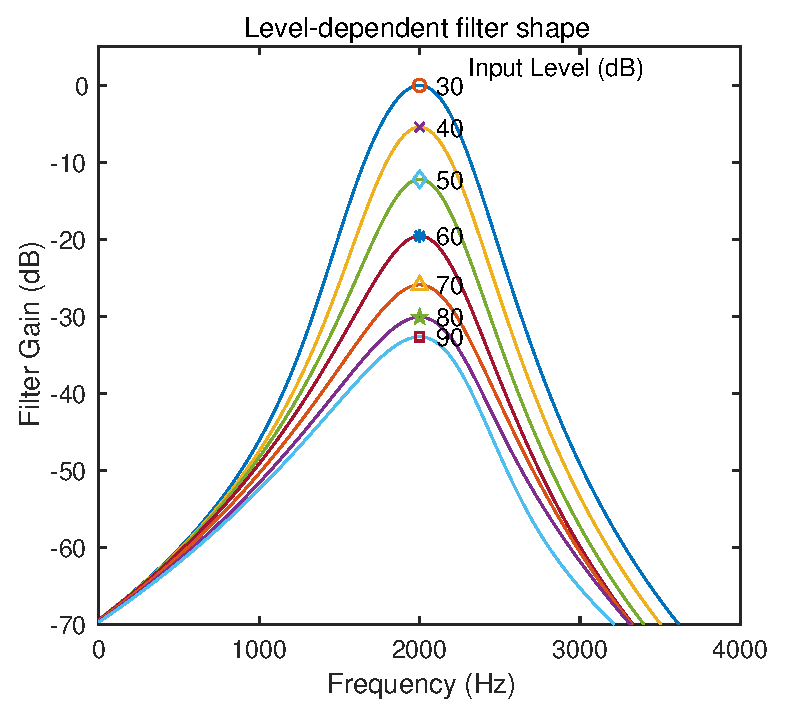
\includegraphics[width=\linewidth]{Figure/RelatedResearch/DemoAF_Basic_FilterLevelDepend.eps}
        \subcaption{音圧依存性}
        \label{fig:Basic_FilterLevelDepend}
    \end{minipage}
    % ---------------------------------------
    \begin{minipage}[t]{0.5\hsize}
        \vspace{50pt}
        \centering
        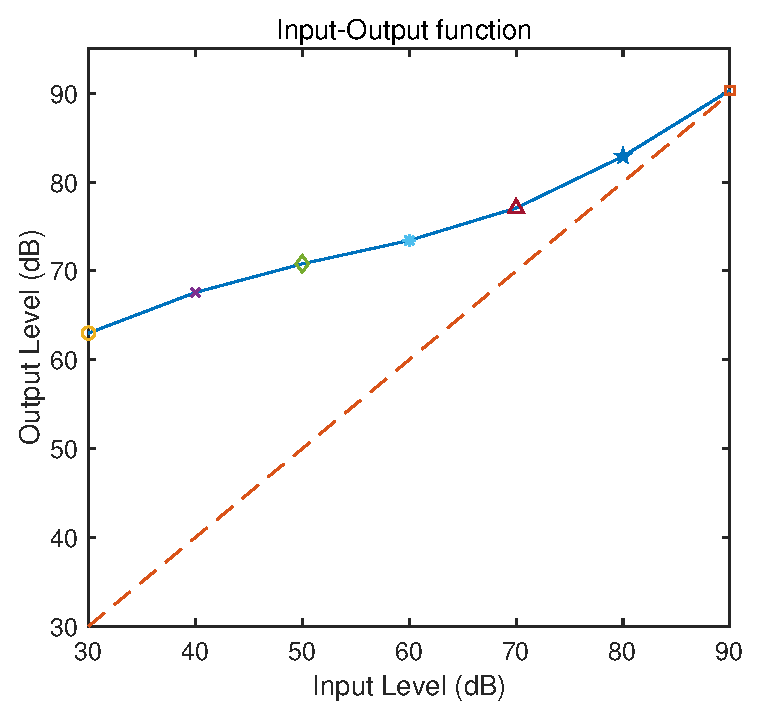
\includegraphics[width=0.96\linewidth]{Figure/RelatedResearch/DemoAF_Basic_IOfunc.eps}
        \subcaption{入出力特性}
        \label{fig:Basic_IOfunc}
    \end{minipage}
    \label{compression}
    % ------------------------------------------
    \caption{聴覚フィルタの音圧依存性(左)と入出力特性(右)の例。図中の記号と色は対応している。
              文献\cite{yamamoto2023GESI}の図2.4より引用。}
\end{figure}
% --------------------------------------------

\newpage



% フィルタ形状の推定〜ガンマチャープフィルタ は略

\clearpage
 % ==============================
\section{\textcolor{red}{時間分析機能, TMTFについても入れたい}}
% \label{sec:peripheral}
% ==============================
音声や音楽など、日常生活のほぼ全ての音は時間的に変動している。そして、その時間変動のパターンの中から、聴覚系は音源や環境に関する情報を取り出している。
時間変動に含まれる情報は、末梢系の周波数分析を経た中枢系において行われている。具体的なメカニズムに関しては、十分に理解が進んでいるとは言えず、あくまで暫定的な仮説に基づいたアプローチが広く用いられている。

聴覚フィルタの出力波形は振幅包絡(変調波)と時間微細構造(temporal fine structure; TFS; 搬送波) のふたつの成分に分類して考えられる。
一般に、音声の時間微細構造をなくして、振幅包絡情報だけで音声知覚ができることが示されている。
ピッチ知覚や両耳間時間差に基づいた音源の分離(たとえば音源定位)においては、TFSの情報が重要である。

% ---------------------------------------
\begin{figure}[h]
    \vspace{40pt}
    \hspace{20pt}
    \centering
    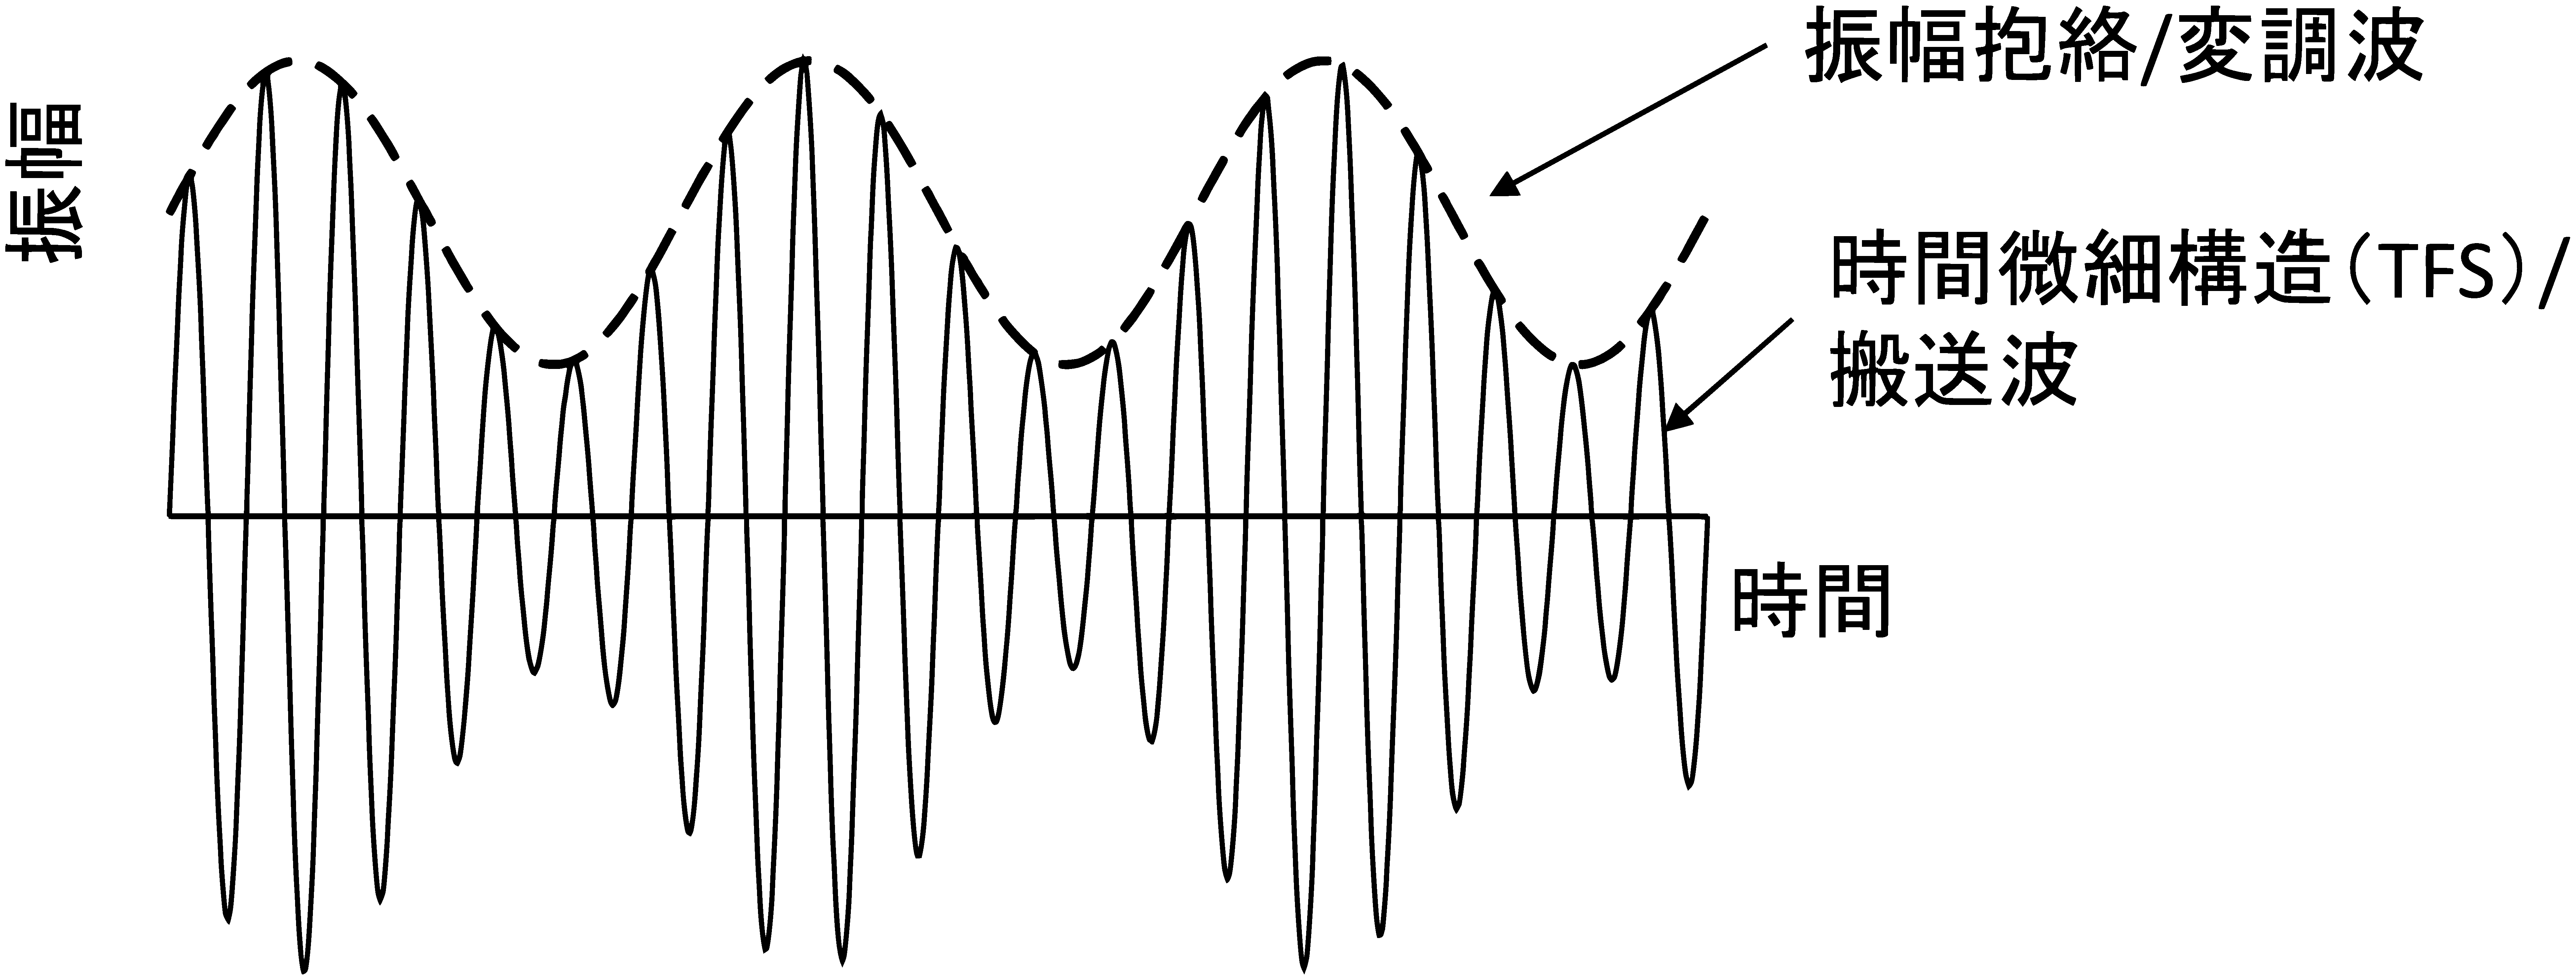
\includegraphics[width=0.8\hsize]{Figure/RelatedResearch/furukawa2016time.eps}
    \caption{振幅包絡と時間微細構造。文献\cite{furukawa2016time}の図1より引用。}
\end{figure}
% --------------------------------------------

% 変調フィルタバンク は略


\clearpage
% ==============================
\section{高齢者の聴覚特性}
% ==============================
高齢になると多くの人が加齢性難聴に悩む。
加齢性難聴の最も深刻な問題が、音声聴取が困難になること、つまり相手の声は聞こえても何を言っているのか理解できない状況である。
この状況がひどくなり、音声コミュニケーションが困難になると社会的生活活動に支障が生じ、社会的孤立、うつ、自己評価の低下につながるかもしれない。

% ------------------------------
\subsubsection{難聴の種類}
% ------------------------------
難聴には、聴覚機能が行なわれた原因によって分類される。
それぞれの特徴を以下にまとめる。

\begin{itemize}
\item \textbf{伝音性難聴 (conductive hearing loss)}\\
 外耳および中耳に機械的障害が生じることにより発生する。
 鼓膜や中耳の耳小骨(つち骨、きぬた骨、あぶみ骨)の損傷が一般的である。
 損傷の部位やその程度にもよるが、聞き取りにくい周波数や聴力レベルは多様であるが、純音聴力が70dBHLを超えることはない。
 エネルギーの大きな音は骨導音として内耳に伝達するためである。
\item \textbf{感音性難聴}\\
 内耳に障害が生じることにより発生する。
 部位ごとに区別され、蝸牛の有毛細胞や聴神経の障害による内耳性難聴(cochler hearing loss)と聴神経系に障害を生じる後迷路難聴(retrocochler hearing loss)がある。
\end{itemize}


% ------------------------------
\subsubsection{加齢性難聴の生理学的要因}
% -----------------------------
加齢性難聴は、末梢系にも中枢系にも要因があると考えられている。
末梢系については大まかに以下の4種類に分類されている\cite{Schuknecht1993presbycusis}。
\begin{itemize}
\item 感覚細胞系:蝸牛内の内有毛細胞・外有毛細胞・支持細胞の損傷
\item 神経細胞系:蝸牛の求心性ニューロンの損傷
\item 代謝系:蝸牛側壁や血管条の萎縮
\item 機械系:基底膜やコルチ器の硬化
\end{itemize}
ただし、これらの要因が混じりあったり、不明な要因による機能低下も存在する。
高齢者に多い高い周波数領域の聴力損失は、蝸牛の有毛細胞の損傷・消失が主な原因となっている。
% ヒトは日常生活において長い間騒音にさらされており、有毛細胞の損傷・消失の大きな原因となっているが、静かな場所で育った動物においても老化の影響があり、有毛細胞は消失していく。



\clearpage
% ------------------------------
\subsubsection{高齢者の純音閾値の周波数特性}
% -----------------------------
さまざまな周波数の純音に対する聴取者の最小可聴閾値(聴覚閾値)の測定は、純音聴力検査(pure tone audiometry)と呼ばれ、
オージオメータ(audio meter)により125, 250, 500, 1000, 2000, 4000, 8000Hzの7つの周波数の純音に対して測定が行われる。
測定結果を図として表したものはオージオグラム(audiogram)という。
若年健聴者の正常聴力閾値を基準(0dB)とし、その値より高くなった閾値のレベルをdBで表現する。
この値を聴力レベル(Hearing level; HL)と呼び、その値が大きいほど聴力が低下していることを意味する。

立木らは、通常の社会生活を営む一般社会人男女約1500人を対象にして聴力レベルを測定した\cite{tuiki2003eldery}。
年代ごとの平均値を表示した例を図\ref{fig:Audiogram}に示す。
この図から、年齢の上昇とともに、全体的に聴力が低下していくが、特に高周波数域の聴力低下の程度が著しくなることがわかる。
さらに、聴力損失は年齢を重ねるほど進行速度が加速される傾向がある。

また、音声聴取に特に重要な 500, 1000, 2000, 4000Hzの4周波数に対して、良い方の耳の聴力レベル(dB)の平均値を代表値(4周波数平均聴力レベル)とし、

\begin{equation}
平均聴力レベル = \frac{HL_{\mathrm(500Hz)} + HL_{\mathrm(1000Hz)} + HL_{\mathrm(2000Hz)} + HL_{\mathrm(4000Hz)}}{4}\\
\end{equation}
の式で計算によって求める。
WHO基準(Prevention of blindness and deafness)では、この平均聴力レベルが25 dB以下であれば正常聴力(健聴者)、26--40 dBであれば軽度難聴、
41--60 dBであれば中等度難聴、61--80 dBであれば高度難聴、81 dBであれば重度難聴と定められている。
% ただし、難聴の基準にはさまざまな種類が存在し、平均聴力レベルの算出には4分法と呼ばれる以下のような方法もある。
% \begin{equation}
% 平均聴力レベル = \frac{HL_{\mathrm(500Hz)} + \bigl(HL_{\mathrm(1000Hz)}\bigr)×2 + HL_{\mathrm(2000Hz)}}{4}\\
% \end{equation}

なお、本研究では、従来の感情認識実験\cite{christensen2019effects}に基づき、正常聴力(健聴者)を平均聴力レベルが22 dB以下とした。
% % ---------------------------------------
\begin{figure}[h]
    \centering
    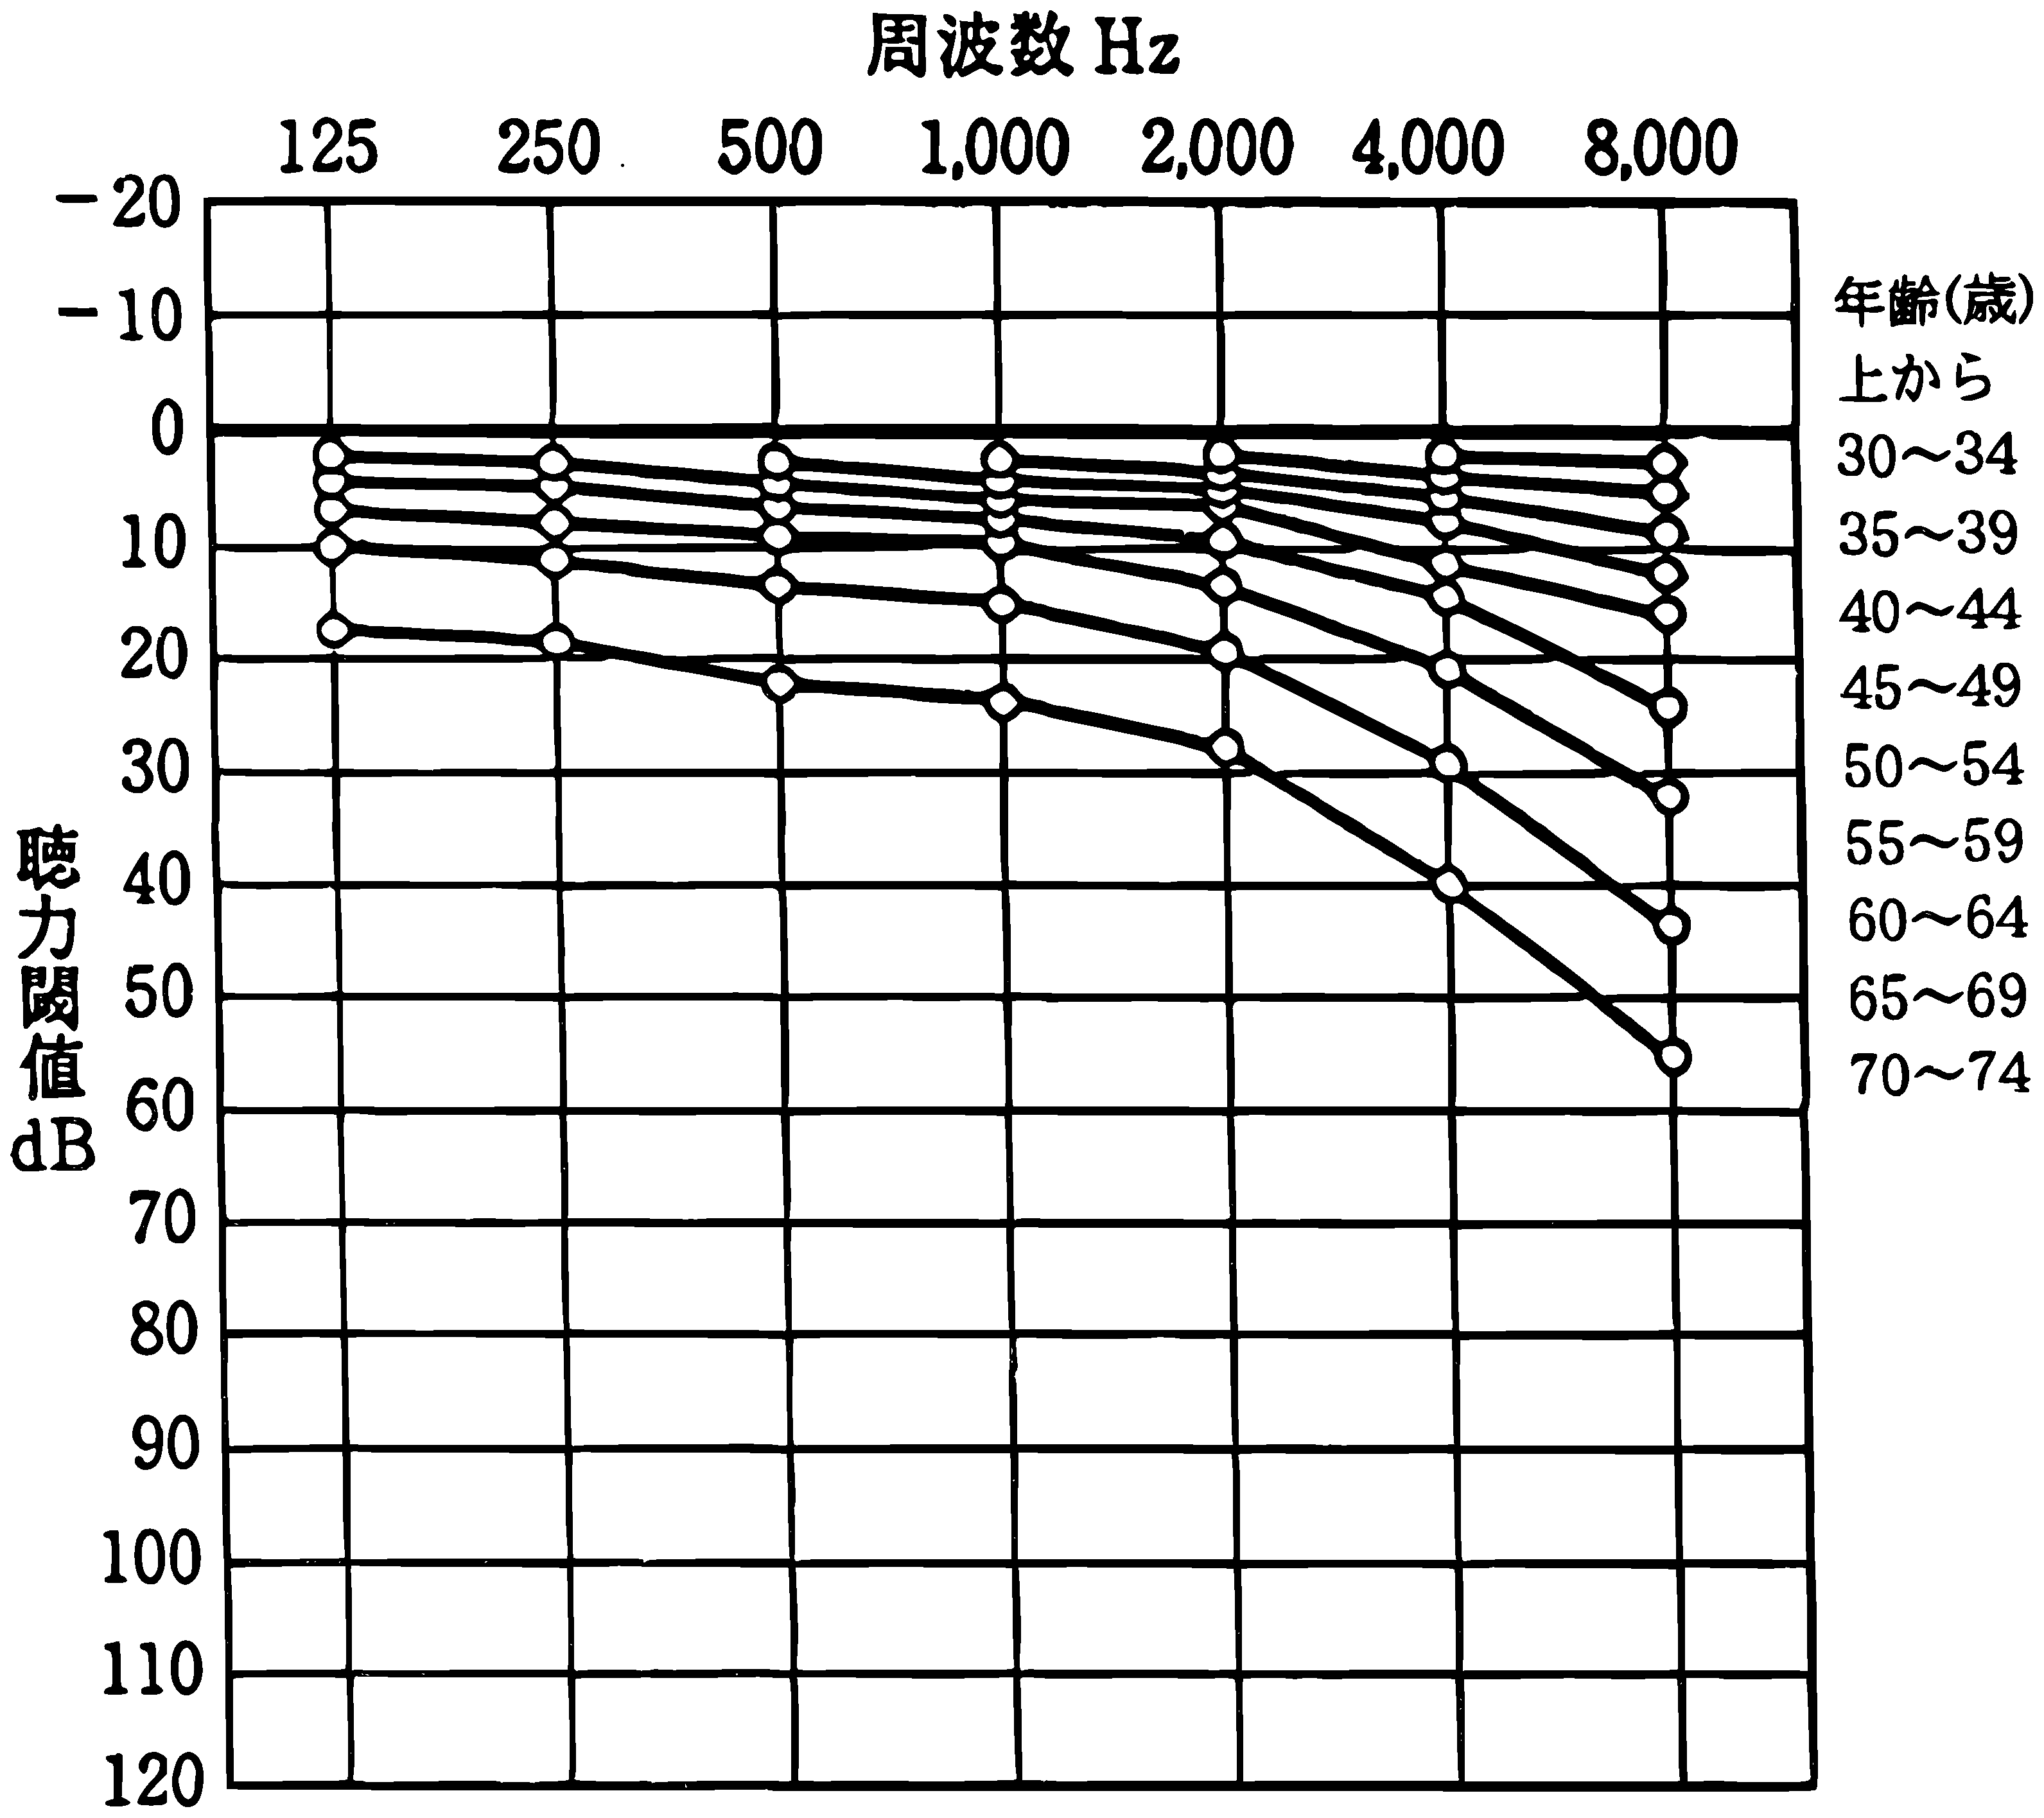
\includegraphics[width=0.6\hsize]{Figure/RelatedResearch/Tsuiki2003Audiogram.eps}
    \caption{年齢別平均オージオグラム(30--74歳, 実測値)。文献\cite{tuiki2003eldery}の図2より引用。}
    \label{fig:Audiogram}
\end{figure}
% % --------------------------------------------



% ------------------------------
\section{模擬難聴システムWHISによる聴覚末梢系の機能低下の模擬 \cite{irino2022moginancho,irino2023hearing}}
\label{sec:WHIS}
% ------------------------------ 
% 模擬難聴とは、健聴者が難聴者の聞こえを体験できる技術である。
% 健聴者が難聴者の困難さを体験できると、難聴者への話しかけ方の改善等につながり、
% 体験型学習や言語聴覚士の養成、患者家族との面談において有用となることが期待されている。
% この模擬難聴は聴覚心理実験に応用されている。
% 難聴者を対象とした聴取実験はこれまでも行われてきたが、難聴者ごとに機能低下の度合いや要因には大きなばらつきがある。
% また、加齢性難聴であれば認知機能の高低も影響する。
% さらに、長時間の聴取実験は集中力維持の観点から難しい。
% そこで、聴覚心理実験において、刺激音を模擬難聴システムを通して若年健聴者が聞くことにより
% 「模擬難聴者」として被験してもらう手法が提案された。
% これにより、認知的問題や集中力問題を回避しつつ、末梢系の特性に関して統制が取れ、
% 少人数でも短時間で明確な結果が得られる可能性が期待されている。

模擬難聴処理システムWHISは、永江らによって開発された健聴者が難聴者の聞こえを体験できる技術である\cite{nagae2016WHIS}。
また、近年WHISの新実装版が開発され\cite{irino2023hearing}、様々な聴覚心理実験に応用されている。


% from ASJ解説25 参照日:26Jan2025,  from irino2022moginancho
高齢難聴者の場合、オージオグラム上の高域で聴力レベルが低下する。
これは、聴覚末梢系の蝸牛における外有毛細胞が担う増幅作用の低下と,振内有毛細胞が担う振動を神経発火に変換する機能の低下の両方の影響による。
前者は入力の広いダイナミックレンジに対してレベル依存する能動的な処理とみなせ、後者は受動的な線形に近い処理とみなせる。
オージオグラムは、それぞれの機能低下の割合を示さず、全体的な閾値上昇だけを示す。
ここで、オージオグラム上の聴力レベル$HL_{total}$は、能動的な聴力損失$HL_{act}$と受動的な聴力損失$HL_{pas}$とのdB上での和で表せると仮定する\cite{moore1997model}。

% 聴覚末梢系の蝸牛においては、外有毛細胞が担う増幅作用と、内有毛細胞が担う振動を神経発火に変換する機能がある。
% 蝸牛以降の機能低下の要因もありうるが、加齢性難聴に限定すれば、ある程度良い近似となっていると考えられる。
WHISでは、この図式を反映できる圧縮型ガンマチャープ聴覚フィルタ\cite{irino2001compressive,irino2006dynamic}を用いている。

% 後者に蝸牛以降の若干の受動的なレベル低下の要因も含めて考えても良いかもしれない。

図\ref{fig:EP_HI=NH+WHIS}に、上記の聴覚モデルを基本とした、模擬難聴処理の概念図を示す。
図\ref{fig:EP_HI=NH+WHIS}(a)に、模擬の対象となる難聴者(HI)の蝸牛の入出力関数を示す。
横軸が入力音圧、縦軸が絶対閾値を0~dBとした励起パターン(EP)のレベルを示している。
一番左の点線は、圧縮特性が健全に機能する健聴者(NH)の入出力関数を示す。
これに対して、レベル依存する能動的な聴力損失は、破線のように入出力関数の傾きを急峻にする。
受動的な聴力損失は入力レベルに依存せず、図中で入出力関数を右側にシフトする。
最終的に、一番右側の一点鎖線の入出力関数になる。
入力音が加わるとこの入出力関数にしたがって、難聴者の励起パターン$EP^{(HI)}$が出力される。
これは、点線の入出力関数が用いられる健聴者(NH)の励起パターン$EP^{(NH)}$よりも小レベルとなる。
WHISでは、健聴者の内部表現としての励起パターンを$EP^{(HI)}$に近づけることを目標とする。
このためには、図\ref{fig:EP_HI=NH+WHIS}(c)に示すように、
能動的なレベル依存の利得低減$R_{act}$と受動的なレベル非依存の利得低減$R_{pas}$を適用することにより、WHISの出力音レベルを減少させる。
これを図\ref{fig:EP_HI=NH+WHIS}(b)に示す健聴者の入出力関数の入力音とすれば、WHISと健聴者特性の両方の特性を反映した$EP^{(NH+WHIS)}$が得られる。
これが$EP^{(HI)}$を十分良く近似できれば、末梢系の機能低下の模擬と見なせるであろう。

上記のとおり現時点のWHISでは、ほぼ末梢系の機能低下の要因だけを模擬している。
そこで、加齢性難聴者と、模擬難聴音を聞く健聴者との対比を行えば、末梢系以降の要因を切り分けて議論できる。
% さらに、たとえば中枢系の時間応答特性の機能低下を模擬難聴に追加できれば、それ以降の特性も推定できる可能性もある。
% ただし、想定した機能低下に対応する音響信号に戻せる定式化を行ったうえで、妥当性と音質の検証をする必要がある。

% 、中枢系のたとえば時間応答特性や認知機能は模擬されていない。

% ----------------------------------%
\begin{figure}[t]
   \vspace{-50pt}
%    \centerline{\includegraphics[width=1.05\linewidth, bb= 0 0 863 803]{Figure/RelatedResearch/Fig_EP_HI=NH+WHIS.eps}}
   \centerline{\includegraphics[width=1.05\linewidth]{Figure/RelatedResearch/Fig_EP_HI=NH+WHIS_v2.eps}}
   \vspace{0pt}
   \caption{蝸牛とシステムの入出力特性の模式図。(a) 難聴者, (b) 健聴者, (c) 模擬難聴システムWHIS。
   入出力関数にしたがって、入力信号は処理され励起パターン(Excitation Pattern, EP)が出力される。難聴者を$EP^{(HI)}$とし、WHISによる模擬難聴出力音を健聴者を聞く場合$EP^{(NH+WHIS)}$とすると、両者の差を小さくすることがWHISの目標となる。文献\cite{irino2023hearing}より引用。
 }
 \vspace{-15pt}
 \label{fig:EP_HI=NH+WHIS}
 \end{figure}
 % ----------------------------------%




\clearpage
%================================================================================================================================
\section{感情音声知覚について}
%================================================================================================================================

% ------------------------------
\subsection{音声と言語\cite{furui1985digital}}
\label{sec:Speech}
% ------------------------------ %参考:東山さん修士論文 
音声は人間が用いるコミュニケーション手段の中で最も基本的なものである。
普段の生活の中でのコミュニケーションにおいて最も重要なのは、相手に伝えたい意味内容、すなわち言語情報である。
またこの音声の中には、話者が誰であるかという個人性情報、話者の感情を表現する情緒性情報など様々な情報が含まれている。
\par
文を形作る基礎は単語(word)であり、各単語は音節(syllable)から成り立ち、音節は音素(phoneme)から成り立つ。
音素には母音(vowel)と子音(consonant)がある。
音節の定義は必ずしも明確ではないが、普通1つの音節は1つの母音もしくは1つの母音と複数の子音が結合してできている。
日本語には、外来語を表現するため特殊なものを除いて101の音節があり、それぞれ仮名と対応している。
日本語には5種類の母音と、分類方法にもよるが、およそ20種類の子音がある。
\par
上述のように、言語学的(音韻論的)な意味での音声の最小基本単位を「音素」と呼び、音声を実際に発声したときに生ずる音声学的な最小基本単位を「単音」と呼ぶ。
前者は音韻記号、後者は音声記号を用いて、それぞれ/a/,[a]というように表す。
\par
アクセント(accent)、強勢(stress)および抑揚(イントネーション;intonation)も言語学的構成の一部であり、音声の強さや高さの時間的変化によって表現される。
アクセントは、連続する音声の中の特定の単語または音節の強さあるいは高さを変えて、他の単語または音声との違いを設け、言葉の意味を明確にする手段である。
強勢はある音節を他よりも強めるためにその音節に加えられる呼気の強さをいう。
イントネーションは、単語や句、文などの言語単位に、その意味、疑問文の区別、強調、話し手の感情などを伝達するために与える声の高さの変化の様相のことをいい、
音調曲線とも呼ばれる。

% ------------------------------
\subsection{感情の心理学論}
\label{sec:PsychoEmo}
% ------------------------------
感情に関する心理学理論は大きく分けて2つある。
1つはエクマンの基本感情説\cite{ekman1992argument}である。
感情はカテゴリー的に存在し、人間の基本感情は「喜び・悲しみ・怒り・恐れ・驚き・嫌悪」の6つに分類できるとしている。
もう1つはラッセルの次元説\cite{russell1980circumplex}であり、感情は「快--不快」の軸と「覚醒--沈静」の軸の
2次元上に円環状に配置されるとしている。
どちらが正しいのか、両者は両立するのか、また両者の関係性については未だによくわかっていない。
ラッセルの感情円環モデルは、感情間の多次元的な関係を2次元平面上に投影したものに過ぎないのかもしれない。
感情間の距離を適切に測定できれば、その関係を多次元構造として研究することが可能になるであろう。


% ------------------------------ 
\subsection{感情音声知覚実験}
\label{sec:PreviousStudy}
% ------------------------------
音声によるコミュニケーションでは、言葉そのもの意味や話の内容といった言語情報だけでなく、性別や年齢など個人の性質や感情、健康状態、声質などの情報が伝達される。
これまでに、音声が感情を伝達する際の音響的特徴についてさまざまな研究が行われてきた。ここではその一部を紹介する。

% note 18~25歳男女55人
白澤らは、6種類の感情(平静・怒り・悲しみ・喜び・驚き・嫌悪)を込めて発話された音声を用いて、話者の意図した感情と聴取者の意図した感情がどの程度一致するかを調査した\cite{shirasawa1996Emo}。
その結果、一致した割合は全体で51.5\%であった。
また、特に悲しみの感情で一致することが多く、喜びでは一致しないことが多かった。
これにより、人間の感情表現や認識力は全ての感情に一様ではなく、偏りがあることが示唆された。

%note 聴覚の健常な日本人大学生・大学院生45名
重野は、「東京」「さようなら」などの単語および短文を用いて、人間の基本6感情(幸福・驚き・怒り・嫌悪・恐れ・悲しみ)を表現した日本語母語話者2名による音声の音響的特徴を分析した\cite{shigeno2004Emo}。
その結果、幸福や驚きなどの「快感情」と判定された発話は、声の平均的高さを表す数値である平均F0が高く、嫌悪などの「不快感情」と判定された発話は平均F0が低いことを明らかにしている。

% 日本または米国在住の4~10歳の児童(モノリンガル)各15名
母語が異なる話者を比較した実験も行われた。
櫻庭らは、日本語または英語を母語とする幼児・児童に感情を込めて/pikachuu/という発話をさせ、日・英語の母語話者にその感情を判断させた\cite{sakuraba2004Emo}。
対象とした感情は喜び・悲しみ・怒り・平静の4つである。その結果、聴者による感情判断には母語による差がないことがわかり、音声による感情は母語に関係なく同様に認知されていることがわかった。
また、日米児の発話を音響分析すると、F0のダイナミックレンジは日米児に共通して感情による変化が見られた。

% 3カ国の出身者。日本:男子大学院生17名。米国:男性11名、女性4名。中国:男子大学生13名
Sawamuraらは、先述の櫻庭らが用いた音声データベース中の怒り・悲しみ・喜びの3感情の音声を用いて聴取実験を行い、発話ごとに含まれる三つの感情成分についてそれぞれ独立に5段階評定をさせた\cite{sawamura2007Emo}。
赤木は、Sawamuraらの実験結果をもとに以下のようにまとめている\cite{akagi2010EmoSpace}。
まず、知覚された感情には度合いがあり、絶対的な数値としての意味を持つものではなく、連続で曖昧な値となる。
また、一つの発話には複数の感情が含まれており、感情の度合いが強ければ一つの感情が知覚されるが、弱ければ複数の感情が知覚される。


% ------------------------------
\subsubsection{加齢による影響}
% ------------------------------
上記の実験に加えて、年齢による感情知覚への影響を検証する実験も行われてきた。
% これまでに、加齢により感情認識精度が低下することが報告されている\cite{paulmann2008aging,ben2019age,amorim2021changes}。

Paulmannらは、$18 \sim 50$歳の男女を対象に、年齢と性別が感情音声認識にどのような影響を与えるか調査した\cite{paulmann2008aging}。
その結果、感情の認識精度は年齢が上がるにつれて低下することが示された。また、性別による差異は見られなかった。

Benらは、話し言葉における感情認識に年齢が与える影響を調査した\cite{ben2019age}。
音声の感情特定については、若年者・高齢者ともに同程度の精度であった。
しかし、音声の感情を評価する場合、若年者は韻律をより重視する一方、
高齢者は韻律と意味をほぼ同程度に考慮し、わずかに意味を重視する傾向があることを示した。

Amorimらは、$7 \sim 82$歳の男女を対象に、音声の感情分類課題を実施した\cite{amorim2021changes}。
その結果、感情認識の精度は小児期から成人期初期にかけて向上し、高齢になるにつれて低下した。

Millらは、$18 \sim 84$歳の男女を対象に、表情または音声の感情認識実験を実施した。
どちらのモダリティにおいてもおおよそ30歳前後から否定的な感情(怒り、特に悲しみ)の認識精度が低下することが示唆された。


%-----------
\subsection{\textcolor{red}{内容ちょっと変える:弁別実験と模擬難聴}}
%-----------
上述のような感情認識実験では感情間の識別境界はわかるものの、感情がどの程度弁別できるかは議論できない。
このためには弁別実験を行って心理物理曲線を求め、弁別閾(JND)や主観的等価点(PSE)を出す必要がある。
しかし、感情弁別実験はほとんど行われていない。
文献\cite{laukka2005categorical}では、Praat\cite{boersma2001speak}を用いて2感情間で、スペクトル・基本周波数・時間間隔を調整して合成した音声を用いた弁別実験を実施していた。
そこで、弁別特性を示す心理物理曲線が得られたが、若年健聴者と高齢者の対比は行われていなかった。
他に見つからないのは、自然音声で2つの感情音声間の刺激連続体を準備することが困難なため合成音声を使わざるをえないが、
その品質や信憑性に疑問が残るのが問題となったからかもしれない。
一方、模擬難聴を用いた実験も存在するが、怒りの感情同定\cite{morgan2022perceived}だけで、感情間の弁別特性はわからなかった。

その研究\cite{laukka2005categorical}から時代を経て、最近では音声間のモーフィングが比較的高品質に実行できる環境が整ってきた\cite{matsui2003STRAIGHT,kawahara2024interactive}。
そこで、モーフィングで合成した音声を用いた感情弁別実験が実施された。
%一人の話者の同一単語で異なる感情音声の間の音声を

% ------------------------------
\subsubsection{音声モーフィングを用いた弁別実験}
% ------------------------------
坂本らは、STRAIGHTに基づいた音声モーフィング技術\cite{matsui2003STRAIGHT}によって合成された感情音声を用いた聴取実験を行なった\cite{sakamoto2020morphEmo}。
ここでは、「平静」と「怒り」の感情で発話された男声と女声それぞれ1名の「はい」が原音声として用いられた。
これらの音声のモーフィング率に対して、聴取者が「怒り」の感情をどの程度知覚するのか調査された。
その結果、全体の傾向としてモーフィングの「怒り」割合に対して、知覚された「怒り」割合は単調増加することが示された。
一方で、モーフィングの「平静」割合が大きいにもかかわらず「怒り」だと知覚されるケースが一定数見られた。

同様に、「平静」と「喜び」、「怒り」と「喜び」の感情音声間での検討もそれぞれ行われた\cite{sakamoto2021morphEmo}。
その結果、平静・怒り音声間での実験と同様に、モーフィング率と知覚される感情の割合に単調増加の傾向が見られた。
平静・喜び音声間での実験では、男声の方が女声よりもJNDの値が大きく、平静と喜びの区別がつきにくいことが示唆された。
怒り・喜び音声間の実験では、女声の場合において怒り感情を判定させた場合と喜び感情を判定させた場合で異なる結果が得られた。

両方の実験で、モーフィング率に対して知覚される感情の割合には個人差が見られた。
また、感情判断には原音声の性別・基本周波数(F0)などの特性や、判定方法が影響している可能性が指摘された。


これらの先行研究\cite{sakamoto2021morphEmo,sakamoto2021morphEmo}の結果を受けて、著者はまだ調査されていなかった「喜び」と「悲しみ」間の弁別実験を実施した\cite{hanatani2023Emo}。
ここでは、先行研究\cite{sakamoto2021morphEmo,sakamoto2021morphEmo}では導入されていなかった模擬難聴処理を導入し、若年健聴者を対象に模擬難聴の有無で感情弁別精度に差異があるかを調査した。
その結果、模擬難聴は感情弁別にほとんど影響しないことが示唆された。
しかし、実験参加者によっては、通常音声がそもそも「喜び」「悲しみ」に感じられなかった、あるいは実験手法を理解できていなかったことが懸念された。
また、使用した音声が男女1名ずつの「はい」という単語1つだけであったことが問題として挙げられた。

そこで、新たな音声データベースを使用し、単語数を増やして同様な弁別実験を実施することにした。
本研究では、先行研究\cite{hanatani2023Emo}の手順を踏襲しつつ、最新の音声モーフィング技術\cite{kawahara2024interactive}を用いた感情弁別実験を実施する。
さらに、これらの研究では行われていなかった聴取者の年齢による影響の有無についての調査も行う。



% ------------------------------ 
\subsection{音声モーフィング}
\label{sec:morphing}
% ------------------------------
モーフィングとは、与えられた2つの事例から、それらの事例の中間に当たるものを作り出すことをいう。
音声モーフィングを用いると、例えば、怒りの感情のこもった音声試料と、悲しみの感情のこもった音声試料から、それらを7対3の割合で混合した音声を合成することができる。
音声モーフィングは感情音声の研究のみならず、歌唱音声などさまざまな研究に応用されている\cite{kawahara2009tandem}。

声の個性や感情、パラ言語情報などの声による多様な表現の理解を深めるためには、収録された音声資料の続計的分析と併せて、
探索的手法による仮説形成と加工音声を用いた主観評価実験による検証を進める必要がある。
音声モーフィング技術は、このような研究を進めるための手段となる。
また、モーフィングにより刺激連続体を作り、それを物差しとして知覚の残効を調べることで背景にある処理モジュールを調べる方法も、利用法の一つとして提案されている。

河原らは、高品質音声分析変換合成法STRAIGHT\cite{kawahara1999restructuring}に基づいた音声モーフィング技術を開発した\cite{matsui2003STRAIGHT}。
また、この技術は刷新され、任意の個数の音声資料を一回の処理でモーフィングすることが可能となった\cite{kawahara2013morph,kawahara2014morph}。
% \ref{sec:先行研究}項で述べる先行研究では、このような技術を使用して作成された実験刺激音が用いられている。

さらに、近年、音声分析合成基盤WORLD\cite{morise2016world}を基盤とした、基本的な音声分析合成の支援や対話的なパラメタ操作による知覚的影響の確認などを容易にするGUIの開発が試みられている\cite{kawahara2024interactive}。
これにはモーフィング音声の合成を支援するツールが含まれている。
本実験では、このツール群を用いて実験刺激音を作成した。
詳しい合成手順は付録\ref{sec:MorphingAppendix}で述べる。



% %\ 感情について
% %SciRep
% 難聴(HL)を抱える高齢者の数は多くの国で増加している。
% 難聴による対人コミュニケーションの低下は、生活の質(QOL)を低下させるだけでなく、認知症の極めて高い危険因子であることが示されている1。
% 音声は、言語的内容と、話し手の特徴や感情を含む副言語的情報の両方を伝えます。
% 従来の補聴器は、主に音声の明瞭度を向上させるように設計されており、感情的なコミュニケーションを改善するものではない。
% 音声の感情認識2-5とその加齢効果6-14に関する研究は数多く行われており、加齢とともに感情認識・識別能力が低下することが報告されている。
% 補聴器は明瞭度を向上させるにもかかわらず、感情認識を向上させないことが確認されている9。
% 加齢は、蝸牛から中枢神経系に至る聴覚プロセスに影響を及ぼす。
% 一つの研究課題は、加齢に関連した末梢の高音域が感情認知にどの程度影響するのか、また異なる段階でどのようなプロセスが関与するのかということである。
% もう一つの疑問は、感情知覚をサポートする新しい補聴器を開発できるかどうかということである。
% 感情の低下が、認知のみによるのではなく、主に音声の特徴や声の表情の聴覚的表現の劣化によって引き起こされるのであれば、新しい強化アルゴリズムを開発することも可能であろう。

% % 感情に関する心理学理論は大きく分けて2つある: 
% % エクマンの基本感情理論では、感情はカテゴリー的に存在するとし、ラッセルの中核感情理論16では、感情は心理的空間の次元に位置するとする。
% % どちらが正しいのか、両者は両立するのか、両者の関係はどうなっているのか、いまだに不明である。
% % ラッセルの2次元モデルは、感情間の多次元的な関係を投影したものに過ぎないのかもしれない。
% % 感情間の距離を適切に測定できれば、その関係を多次元構造として研究することが可能になる。
% % このアプローチの重要な点は、多次元構造を比較することにより、老若男女間の年齢効果を調べることができること、
% また、その結果を補聴器の新しいアルゴリズムを開発するための感情知覚の聴覚モデルを構築する際の重要な制約条件として用いることができることであろう。
% % 知覚距離の推定には、感情認識性能6-14ではなく、感情ペア間のカテゴリー知覚の心理測定関数4が使えると仮定した。

% %
% % しかし、異なる感情間の刺激の連続性を用意することが不可欠であり、人間の自然な音声でこれを実現することはほとんど不可能である。
% %  音声モーフィングを使ったこのような実験の初期の試みがある4。
% % モーフィングされた特徴は、基本周波数のF0、音素のタイミング、強弱に限定されていたが、当時知られていた技術を考えると、これは良いアプローチであった。
% % しかし現在では、高品質の音声分析・修正・合成システムであるSTRAIGHT17,18や、その後継システムであるWORLD19を用いて、より優れた実験刺激を作成できるようになりました。
% % 例えば、スピーカーの大きさを知覚する実験20,21が行われ、聴覚モデルの制約に用いられています22。
% % これらの実験での音声修飾は、平滑化されたスペクトログラムの比較的単純なスペクトルの拡張と収縮によって行われたが、GUIを備えた最近の音声モーフィングツール23を使用して、対応する特徴点を正しく割り当てれば、
% % 同じ単語の2つの音声の中間音を生成することも可能である。


% % ------------------------------ 
% \subsection{音声の感情知覚}
% \label{sec:音声の感情知覚}
% % ------------------------------
% 音声によるコミュニケーションでは、言葉そのもの意味や話の内容といった言語情報だけでなく、性別や年齢など個人の性質や感情、健康状態、声質などの情報が伝達される。
% これまでに、音声が感情を伝達する際の音響的特徴についてさまざまな研究が行われてきた。

% 白澤らは、6種類の感情(平静・怒り・悲しみ・喜び・驚き・嫌悪)を込めて発話された音声を用いて、話者の意図した感情と聴取者の意図した感情がどの程度一致するかを調査した\cite{shirasawa1996Emo}。
% その結果、一致した割合は全体で51.5\%であった。
% また、特に悲しみの感情で一致することが多く、喜びでは一致しないことが多かった。
% これにより、人間の感情表現や認識力は全ての感情に一様ではなく、偏りがあることが示唆された。

% 重野は、「東京」「さようなら」などの単語および短文を用いて、人間の六つの基本感情(幸福・驚き・怒り・嫌悪・恐れ・悲しみ)を表現した日本語母語話者2名による音声の音響的特徴を分析した\cite{shigeno2004Emo}。
% その結果、幸福や驚きなどの「快感情」と判定された発話は、声の平均的高さを表す数値である平均F0が高く、嫌悪などの「不快感情」と判定された発話は平均F0が低いことを明らかにしている。

% 母語が異なる話者を比較した実験も行われた。
% 櫻庭らは、日本語または英語を母語とする幼児・児童に感情を込めて/pikachuu/という発話をさせ、日・英語の母語話者にその感情を判断させた\cite{sakuraba2004Emo}。
% 対象とした感情は喜び・悲しみ・怒り・平静の4つである。その結果、聴者による感情判断には母語による差がないことがわかり、音声による感情は母語に関係なく同様に認知されていることがわかった。
% また、日米児の発話を音響分析すると、F0のダイナミックレンジは日米児に共通して感情による変化が見られた。

% Sawamuraらは、先述の櫻庭らが用いた音声データベース中の怒り・悲しみ・喜びの3感情の音声を用いて聴取実験を行い、発話ごとに含まれる三つの感情成分についてそれぞれ独立に5段階評定をさせた\cite{sawamura2007Emo}。
% 赤木は、Sawamuraらの実験結果をもとに以下のようにまとめている\cite{akagi2010Emo}。
% まず、知覚された感情には度合いがあり、絶対的な数値としての意味を持つものではなく、連続で曖昧な値となる。
% また、一つの発話には複数の感情が含まれており、感情の度合いが強ければ一つの感情が知覚されるが、弱ければ複数の感情が知覚される。








% % ------------------------------ 
% \subsection{先行研究}
% \label{sec:先行研究}
% % ------------------------------ 
% % 関連研究にまとめていいかも 海外論文の方も書く
% \ref{sec:音声の感情知覚}項で述べた研究で用いられた感情音声は、表現する感情を明確に意図して発話された音声であり、曖昧な感情音声は用いられていない。
% 先行研究では、このような曖昧な感情音声について人間がどのような感情をどの程度知覚するかの調査が行われた。

% 坂本らは、STRAIGHTに基づいた音声モーフィング技術\cite{matsui2003STRAIGHT}によって合成された感情音声を用いた聴取実験を行なった\cite{sakamoto2020morphEmo}。
% ここでは、「平静」と「怒り」の感情で発話された男声と女声それぞれの「はい」が原音声として用いられた。
% これらの音声のモーフィング率に対して、聴取者が「怒り」の感情をどの程度知覚するのか調査された。
% その結果、全体の傾向としてモーフィングの「怒り」割合に対して、知覚された「怒り」割合は単調増加することが示された。
% 一方で、モーフィングの「平静」割合が大きいにもかかわらず「怒り」だと知覚されるケースが一定数見られた。

% 同様に、「平静」と「喜び」、「怒り」と「喜び」の感情音声間での検討もそれぞれ行われた\cite{sakamoto2021morphEmo}。
% その結果、平静・怒り音声間での実験と同様に、モーフィング率と知覚される感情の割合に単調増加の傾向が見られた。
% 平静・喜び音声間での実験では、男声の方が女声よりもJNDの値が大きく、平静と喜びの区別がつきにくいことが示唆された。
% 怒り・喜び音声間の実験では、女声の場合において怒り感情を判定させた場合と喜び感情を判定させた場合で異なる結果が得られた。

% 全ての実験で、モーフィング率に対して知覚される感情の割合には個人差が見られた。
% また、感情判断には原音声の性別・基本周波数(F0)などの特性や、判定方法が影響している可能性が指摘された。




\newpage
%%%%%%%%%%%%%%%%%%%%%%%%%%%%%%%%%%%%%%%%%%%%%%%%%%%%%%%%%%%%%%%%%%%%%%%%%%%%%%%%%%
%%%%%%%%%%%%%%%%%%%%%%%%%%%%%%%%%%%%%%%%%%%%%%%%%%%%%%%%%%%%%%%%%%%%%%%%%%%%%%%%%%
\chapter{怒り・悲しみ・喜び間の弁別実験}
\label{chap:ExpAngHapSad}
%%%%%%%%%%%%%%%%%%%%%%%%%%%%%%%%%%%%%%%%%%%%%%%%%%%%%%%%%%%%%%%%%%%%%%%%%%%%%%%%%%
%%%%%%%%%%%%%%%%%%%%%%%%%%%%%%%%%%%%%%%%%%%%%%%%%%%%%%%%%%%%%%%%%%%%%%%%%%%%%%%%%%

高齢難聴者の感情音声知覚特性を調べるために、「怒り」「悲しみ」「喜び」の3感情間のモーフィング音声を用いて、
若年健聴者と高齢者を対象にした感情弁別実験を実施した。
先行研究\cite{hanatani2023Emo}の結果を受けて、複数の単語が収録された新たな音声データベース\cite{keioESD-J}を使用した。
まず、聴覚末梢系の機能低下だけが感情知覚に与える影響を調べるために、若年健聴者には模擬難聴処理を行った音声を聴かせて、
通常音声を聴いた場合との感情知覚の相違を検討する。
次に、高齢者にも同じ通常音声を用いて実験を行い、若年健聴者の結果と比較する。

ここでは、はじめに実験刺激の作成方法と実験手順、実験条件について説明する。
その上で、若年健聴者・高齢者の実験結果をそれぞれ示し、結果を比較する。
若年健聴者が通常音声を聞いた場合、同じ若年健聴者が模擬難聴音を聞いた場合、高齢者が同じ通常音声を聞いた場合の
弁別精度を比較し、これら3つの条件の違いから、高齢者の感情知覚の特徴について調査していく。

% ------------------------------
\section{実験刺激の作成}
\label{sec:PrepareStimuli}
% ------------------------------
感情を最もよく表現する音声の抽出を行い、音声モーフィングと模擬難聴処理で実験刺激を作成した。

% ------------------------------
\subsubsection{感情音声の再分類 \textcolor{red}{付録にスクリーニング結果入れる?}}
% ------------------------------
使用した音声データベースは慶應義塾大学研究用感情音声データベース(Keio-ESD)\cite{keioESD-J}である。
このデータベースには、舞台経験のある一般人男性(32歳)1名が、20単語それぞれを47通りの感情(以下では元感情と呼ぶ)で発声した940音声に、
複数回発声の平静音声を加えて全1025音声が収録されている。
そのうち、名詞11単語(「なみ」「なま」「みどり」「ななめ」「ながめ」「あまみず」「おもなが」「あまのがわ」「あまりもの」「おぼろづきよ」「わらわれもの」)を用いることとした。

47種ある感情を話者がどの程度表現できているか、音声を聞いて本当にその感情らしく感じられるかを確かめるために、
実験者3名(著者を含む若年健聴者:日本人大学生と大学院生)で音声の再分類を行った。
47元感情・11単語の音声を全て聞き、エクマンの基本6感情(喜び・悲しみ・怒り・恐怖・嫌悪・驚き)\cite{ekman1992argument}に分類した。
この中から、「怒り」「悲しみ」「喜び」に分類された音声は176音声(11単語 $\times$ 16元感情)であった。
この3つの感情を選択した理由は、多くの研究で一般的に用いられていて、本研究のアプローチの第一歩として適していると考えたためである。

\newpage


% ------------------------------
\subsubsection{感情尺度評定と主成分分析}
% ------------------------------
抽出された176音声の感情の強さを測定するために、前述の実験者3名が基本6感情について5段階の尺度評定を行った。
評定を行った理由としては、この段階までで大まかに感情カテゴリーごとに分かれているが、「怒り」「悲しみ」「喜び」以外の感情も知覚される可能性があるためである。
その上で、全音声・実験者3名の6感情の評定値を変数として主成分分析を行った。
この結果の第1主成分(PC1)と第2主成分(PC2)の分布を図\ref{fig:PCA-Russel_AngHapSad}(a)に示す。

PC2まで、累積寄与率84\%を占めた。
この図では、図\ref{fig:PCA-Russel_AngHapSad}(b)に示すラッセルの円環モデル\cite{russell1980circumplex}内の感情語の位置となるべく近くなるように配置を調整した。
横軸をPC2、縦軸にPC1の符号を反転させたものとしている。
比較すると、PC2が快--不快の軸で、PC1の逆符号が覚醒--沈静の軸とおおまかに一致することがわかる。
また、中心から三角形の頂点に向かう線に沿うように分布している。
各単語ごとに、三角形の頂点に近く原点から離れた音声、つまり最も「怒り」「悲しみ」「喜び」らしい単語を16元感情の中から抽出した。
これで同一内容の11単語を3感情分、合計33音声をそろえた。
なお、薄い線の三角形は、抽出された音声を単語ごとに結んでいる(次のセクションで説明する1単語を除く)。


%%%%%%%%%%%%%%%%%%%%%% %%%%%%%%%%%%%%%%%%%%% %%%%%%%%%%%%%%%%%%%%% 
% 主成分分析結果・Russel  Ang-Hap-Sad

\begin{figure}[t]

  \begin{tabular}{cc}
  \begin{minipage} {0.47\hsize}
  \centering
  \includegraphics [ width = 1\columnwidth]{Figure/ExpAngHapSad/FigPCA_CumAll_scatter_SndTriangle_Eng.eps}
  \end{minipage} & 
  
  \begin{minipage} {0.47\hsize}
  \centering
  \includegraphics [ width = 1\columnwidth]{Figure/ExpAngHapSad/Fig_RusselCircle_b.eps }
  \end{minipage}
  
  \end{tabular}
  
  \caption{感情尺度評定の主成分分析(PCA)結果(a)とラッセルの感情円環モデル(b)(\cite{russell1980circumplex}のFig.4より再描画)。
            図(a)の各点(x)は、単語ごとに基本6感情("Ang"怒り,"Sad"悲しみ,"Hap"喜び,"Fea"恐怖,"Dis"嫌悪,"Sur"驚き)の評価を行って得られたPCAスコアを示す。
            薄い線の三角形は抽出された10単語それぞれを結ぶ。
            ラッセルの円環モデル(b)内の感情との位置関係に合わせるため、横軸をPC2、縦軸をPC1の符号反転としている。
            }
  \label{fig:PCA-Russel_AngHapSad} 

\end{figure}




% \newpage
% ------------------------------
\subsubsection{音声モーフィング}
% ------------------------------

抽出した33音声(11単語\time 3感情)について、
音声分析変換合成システムWORLD\cite{morise2016world}を用いた音声モーフィング用のGUI\cite{kawahara2024interactive}で、
感情間の中間の音声を合成した。
図\ref{fig:MorphingAligner}に、例として単語「なみ」の喜び音声と悲しみ音声のWORLDスペクトルと、モーフィングのための特徴点を示す。

まず、GUI上で図\ref{fig:MorphingAligner}左のように一方のスペクトルを表示し、音声の音響的に異なる領域の境界を手動で設定する(縦の薄い白線)。
次に、各境界線上でレベルが大きい部分に特徴点を手動で指定する。
その後、この特徴点表示を残したままもう一方のスペクトルをオーバーレイ表示させる。
そこでこれらの点を、オーバーレイ表示させたスペクトルのレベルが大きい部分に、図\ref{fig:MorphingAligner}右になるように移動させる。
その上で、モーフィング率を指定して実行すると、この2つのスペクトル間を線形補完するようにスペクトル変形がなされ合成音が生成される。
ここでは、モーフィング率が 0,20,40,50,60,80,100\%の音声を合成した(0\%, 100\%の音声も分析合成系の影響を入れ込むため、合成している)。
合成した音声を聞き、モーフィング音声の劣化がなるべく小さくなるように特徴点の位置を繰り返し調整した。
実験者3名で、3組の感情対(「怒り-悲しみ」「悲しみ-喜び」「喜び-怒り」)を分担して作業を行った。
最後に、全員が全ての合成音を聴取し、音質の確認を行った。
確認した結果、1単語「おぼろづきよ」は他の単語よりモーフィングの際の劣化が目立ち、歪みを小さくすることができなかった。
% また、感情単語として使われる状況を想像しやすいとは思えない。
そこで、残りの10単語を実験刺激として用いることとした。
これにより、10単語\time 7モーフィング率\time 3感情間の合計210音声を準備した。
\textcolor{red}{図4にその音声の配置の概念図を示す。}


% これは、恒定法で一対比較を行い感情知覚の弁別閾を求めるためである。 
% ちょうど中間の50\%の音声に対し、他のモーフィング率の音声を比較させ、どちらが指定した感情(たとえば「喜び」)に感じるかを回答させる。
% これを3組の感情対に関して11単語分作成した。


%%%%%%%%%%%%%%%%%%%%%% %%%%%%%%%%%%%%%%%%%%% %%%%%%%%%%%%%%%%%%%%% 
% MorphingAligner スクリーンショット
% 単語 nami の喜び-悲しみ

\begin{figure}[t]

  \begin{tabular}{cc}
  \begin{minipage} {0.47\hsize}
  \centering
  \includegraphics [ width = 1\columnwidth]{Figure/ExpAngHapSad/Fig_nami_hap_Spect.eps}
  \end{minipage} & 
  
  \begin{minipage} {0.47\hsize}
  \centering
  \includegraphics [ width = 1\columnwidth]{Figure/ExpAngHapSad/Fig_nami_sad_Spect.eps }
  \end{minipage}
  
  \end{tabular}
  
  \caption{単語「なみ」のWORLDスペクトル。左: 喜び音声、右: 悲しみ音声。それぞれモーフィングのための特徴点を白点で示す。文献 \cite{hanatani2024onsei}の図3から引用。}
  
  \label{fig:MorphingAligner} 

\end{figure}



% ------------------------------
\subsubsection{模擬難聴処理}
% ------------------------------

\ref{sec:研究目的}節で述べたように、若年健聴者実験では通常音声と模擬難聴音声の対比を行う。
モーフィングで合成した上記の210音声(以下では、無処理の意味で"Unpro"と呼ぶ)と対比するために、
模擬難聴システムWHIS\cite{irino2023hearing}を用いて、模擬難聴音声を作成した。
本実験では、80歳の平均聴力レベル \cite{tsuiki2002nihon_Jpn}、圧縮特性健全度を中程度の$\alpha=0.5$と設定した。
すなわち、125,250,500,1000,2000,4000,8000Hzで、24,24,27,28,33,48,69dBとした。
つまり、500~Hzから4000~Hzの平均聴力レベルは34dBである。
得られた210個の模擬難聴音声を、以降"80yr"と呼ぶ。


\newpage
% ------------------------------
\section{実験手順と実験条件}
\label{sec:ExpCondition}
% ------------------------------
前節で述べた実験刺激を用いて、若年健聴者と高齢者を対象に感情弁別実験を行った。
参加者は「怒り--悲しみ」対、「悲しみ--喜び」 対、「喜び--怒り」対の3つの実験すべてに参加した。
実験は和歌山大学の倫理委員会の承認を受けており、実験前に説明を行ってインフォームドコンセントを得た。

実験には恒常法を用い、基準となるモーフィング率50\%の音声(標準刺激)と、その他のモーフィング率の音声(比較刺激)を1対で順番に提示した。
手掛語として表示される感情ラベル(例えば悲しみ)に、どちらの音声が近いかを二肢強制選択で回答させた。
この手掛語(悲しみ)の実験が終わった後、対の手掛語(喜び)の実験を全く同じ刺激を用いて行った。
全ての実験は防音室内で専用のWebページを用いて行った。


% ------------------------------
\subsubsection{若年健聴者実験}
% ------------------------------

若年健聴者実験では、無処理音(Unpro)と模擬難聴音(80yr)の両方を使った。
したがって、刺激対は、10単語$\times$標準刺激と比較刺激の組み合わせ6組$\times$音声処理条件(Unpro/80yr)2条件$\times$提示順のカウンタバランス2条件=240対である。
提示順は基本的に参加者ごとにランダムで、1セッションあたり各12の音声対の全20セッションとした。
ただし、Unproと80yrは音圧が異なるため、別セッションに割り当てることでセッション内ではどちらかの条件に統一されている。

また、感情判断においてバイアスがないかを調べるために、判断させる感情を入れ替えて2回実験した。
具体的に、例えば悲しみ--喜び対の実験で説明する。
まず、全240対の比較において、「悲しみ」という手掛語を提示し、どちらの音声がより「悲しみ」に聞こえるかを判断させた。
その後、全く同じ実験刺激対を用いて、手掛語をもう一方の感情(喜び)に入れ替えて判断させ、反応バイアスがあるかどうかを調べた。
すなわち、1人の実験参加者は、全480対を聴取した。
どちらの手掛語が先かや、どの感情対の実験から始めるかは、参加者間でバランスを取った。

参加者は、20歳から24歳の日本人大学生12名(男性7名、女性5名)であった。
全員が125Hzから8000Hzの範囲で聴力レベルが25\,dB以下で健聴者であることを確認した。


% ------------------------------
\subsubsection{高齢者実験}
% ------------------------------

高齢者実験は若年健聴者実験と手順は同じである。
ただし、Unpro音声だけを実験刺激として、80yrの模擬難聴音は使用しない。
したがって刺激対は、10単語$\times$標準刺激と比較刺激の組み合わせ6組$\times$提示順のカウンタバランス2条件=120対である。
% 健聴者実験の半分なので全10セッションとした。
提示順は基本的にランダムで、1セッションあたり各12の音声対を聞き、全10セッションに分けた。
感情判断に用いる手掛語は若年健聴者実験と同様に2通り設定した。
一方の手掛語の全120対の実験が終了した後、もう一方の手掛語の実験を全く同一の刺激セットで実施した。
すなわち、1人の実験参加者は、全240対を聴取した。
どちらの手掛語から先に始めるかは、全被験者で統一した。
どの感情対の実験から始めるかは、参加者間でバランスを取った。

シルバー人材センターに依頼して実験参加者を募集した。
参加者は61歳から81歳の12名(男性9名・女性3名)である。
参加者のうち2名は、良耳が125Hzから8000Hzの全帯域で聴力レベルが25dB以下であり、健聴レベルであった。
しかし、残りの10名は高齢難聴の傾向があった。
500~Hzから4000~Hzの平均聴力レベルは6.3$\sim$28.8dBであった。


% from Scirep24 高齢者の聴力について
% 図2cの統計分析では、高齢の参加者を聴力レベルに応じてNH群とHL群(ONHとOHL)に分けた。
% ONHは、感情認識研究11の基準に従い、500Hz、1000Hz、2000Hz、4000Hzの聴力レベルの平均が、良い方の耳で22dB以下であると仮定した。
% また、HLシミュレーションの結果、8000Hzの聴力レベルは感情認知に直接影響しない可能性が示唆されたためである。
% その結果、参加者はONHが7人、OHLが5人となった。
%  なお、閾値を25dBに設定した場合でも、図2cの有意な関係は不変であった。 
\newpage
%%%%%%%%%%%%%%%%%%%%%%%%%%%%%%%%%%%%%%%%%%%%%%%%%%%%%%%%%%%%%%%%%%%%%%%%%%%%%%%%%%
%%%%%%%%%%%%%%%%%%%%%%%%%%%%%%%%%%%%%%%%%%%%%%%%%%%%%%%%%%%%%%%%%%%%%%%%%%%%%%%%%%
\chapter{落着きと怒り・悲しみ・喜び間の弁別実験}
\label{chap:ExpCalm}
%%%%%%%%%%%%%%%%%%%%%%%%%%%%%%%%%%%%%%%%%%%%%%%%%%%%%%%%%%%%%%%%%%%%%%%%%%%%%%%%%%
%%%%%%%%%%%%%%%%%%%%%%%%%%%%%%%%%%%%%%%%%%%%%%%%%%%%%%%%%%%%%%%%%%%%%%%%%%%%%%%%%%
第\ref{chap:ExpAngHapSad}章の実験では、高齢者にとって喜び--怒りの判断だけが有意に難しいことがわかった。
そこで、ラッセルの感情円環モデル\cite{russell1980circumplex}との対応関係を用いて考察を進めた。
そして、覚醒度が同程度である場合、快-不快の判断が難しいという作業仮説を立てた。
その上で、ラッセルの円環モデル上で悲しみと快-不快軸上で反対にある「落着き」の音声を使って同様な弁別実験を行った。

ここでは、第\ref{chap:ExpAngHapSad}章と同様の構成で、実験手順・実験条件・実験結果について述べる。
実験結果では、第\ref{chap:ExpAngHapSad}章で行った怒り・悲しみ・喜び間の弁別実験結果と比較することで、作業仮説の検証を行う。

% ------------------------------
\section{実験刺激の作成}
\label{sec:PrepareStimuli_cal}
% ------------------------------
怒り・悲しみ・喜び実験(第\ref{chap:ExpAngHapSad}章)と同様な手順で、「落着き」感情を最もよく表現する音声の抽出を行い、
音声モーフィングと模擬難聴処理で実験刺激を作成した。


% ------------------------------
\subsubsection{「落着き」感情音声の選別}
% ------------------------------
使用した元音声は、怒り・悲しみ・喜び実験と同じ慶應義塾大学研究用感情音声データベース(Keio-ESD)\cite{keioESD-J}である。
用いた単語も同じで、名詞の10単語とした。

今回の実験では、上述の作業仮説を検証するため、「快」かつ「沈静」の感情である「落着き」を新たに導入した。
実験者3名(著者を含む若年健聴者:日本人大学生と大学院生)で47元感情・10単語の音声を再度全て聞き、「落着き」に感じた発声(48音声)を選別した。
この48音声に、怒り・悲しみ・喜び実験で用いた30音声を加えた合計78音声を用いて、次の感情尺度評定を行っていく。
詳細な手続きは付録\ref{sec:DBScreening}にて述べる。

% \newpage


% ------------------------------
\subsubsection{感情尺度評定と主成分分析}
\label{sec:5Scale_Calm}
% ------------------------------
選別した78音声に関して、実験者3名が「怒り」「悲しみ」「喜び」「落着き」の4感情を評定軸とした段階尺度評定を行った。
その上で、全音声・実験者3名の4感情の評定値を変数として主成分分析を行った。
この結果の第3主成分(PC3)までの分布を図\ref{fig:PCA-Russel_Calm}(c)に示す。
PC3までで、累積寄与率99\%を占めた。
図\ref{fig:PCA-Russel_AngHapSad}(a)と同様に、「怒り」「悲しみ」「喜び」の3感情が三角形の頂点付近にそれぞれ分布している。
一方、落着き音声(黒のx印)は3感情とは逆方向に、三角形を底面とした三角錐の頂点の方向に分布している。
各単語ごとに、落着きベクトル(Cal)との内積が最も大きい、つまり最も「落着き」らしい10単語を抽出した。
以上より、同一内容の10単語を4感情分そろえた。


%%%%%%%%%%%%%%%%%%%%%% %%%%%%%%%%%%%%%%%%%%% %%%%%%%%%%%%%%%%%%%%% 
% 主成分分析結果・Russel  Calm

% ---------------------------------------
\begin{figure}[h]
  \vspace{40pt}
  \hspace{20pt}
  \centering
  \includegraphics[width=0.8\hsize]{Figure/ExpCalm/FigPCA3d_CumAll_cal2_scatter_SndTriangle_Eng.eps}
  \caption{感情尺度評定の主成分分析(PCA)結果。各点(x)は、怒り,悲しみ,喜び,落着きの評価を行って得られたPCAスコアを示す。
            "Ang"怒り,"Sad"悲しみ,"Hap"喜び,"Cal"落着き。 見やすさのため3次元で描画している。}
\end{figure}
% --------------------------------------------


% \begin{figure}[t]

%   \begin{tabular}{cc}
%   \begin{minipage} {0.47\hsize}
%   \centering
%   \includegraphics [ width = 1\columnwidth]{Figure/ExpAngHapSad/FigPCA_CumAll_scatter_SndTriangle_Eng.eps}
%   \end{minipage} & 
  
%   \begin{minipage} {0.47\hsize}
%   \centering
%   \includegraphics [ width = 1\columnwidth]{Figure/ExpAngHapSad/Fig_RusselCircle_b.eps }
%   \end{minipage}
  
%   \end{tabular}
  
%   \caption{感情尺度評定の主成分分析(PCA)結果(a)とラッセルの感情円環モデル(b)(\cite{russell1980circumplex}のFig.4より再描画)。
%             図(a)の各点(x)は、単語ごとに基本6感情("Ang"怒り,"Sad"悲しみ,"Hap"喜び,"Fea"恐怖,"Dis"嫌悪,"Sur"驚き)の評価を行って得られたPCAスコアを示す。
%             薄い線の三角形は抽出された10単語それぞれを結ぶ。
%             ラッセルの円環モデル(b)内の感情との位置関係に合わせるため、横軸をPC2、縦軸をPC1の符号反転としている。
%             }
%   \label{fig:PCA-Russel_Calm} 

% \end{figure}




% \newpage
% ------------------------------
\subsubsection{音声モーフィング}
\label{sec:morphCalm}
% ------------------------------

抽出した40音声(10単語$\times$4感情)について、音声モーフィング用のGUI\cite{kawahara2024interactive}を用いて、
「怒り--落着き」「悲しみ--落着き」「喜び--落着き」間の中間の音声を合成した。
合成の手順は怒り・悲しみ・喜び実験と同じで、モーフィング率が0,20,40,50,60,80,100\%の音声を、3つの感情対に関して10単語分作成した。 
図\ref{fig:ExpRsltEmoPercent_Calm}(a)にその音声の配置の概念図を示す。
これにより、10単語$\times$7モーフィング率$\times$3感情対の合計210音声を準備した。

% ------------------------------
\subsubsection{模擬難聴処理}
% ------------------------------

怒り・悲しみ・喜び実験と同様に、若年健聴者実験では通常音声と模擬難聴音声の対比を行う。
模擬難聴システムWHIS\cite{irino2023hearing}を用いて、模擬難聴音声を作成した。
80歳の平均聴力レベル \cite{tsuiki2002nihon_Jpn}、圧縮特性健全度を中程度の$\alpha=0.5$と設定した。


\newpage
% ------------------------------
\section{実験手順と実験条件}
\label{sec:ExpCondition_Calm}
% ------------------------------
前節で述べた実験刺激を用いて、若年健聴者と高齢者を対象として実験を行った。
実験手順は怒り・喜び・悲しみ実験と同じである。
参加者は「怒り--落着き」対、「悲しみ--落着き」対、「喜び--落着き」対の3つの実験すべてに参加した。
実験は和歌山大学の倫理委員会の承認を受けており、実験前に説明を行ってインフォームドコンセントを得た。


% ------------------------------
\subsubsection{若年健聴者実験}
% ------------------------------

若年健聴者実験では、無処理音(Unpro)と模擬難聴音(80yr)の両方を使った。
したがって、刺激対は、10単語$\times$標準刺激と比較刺激の組み合わせ6組$\times$音声処理条件(Unpro/80yr)2条件$\times$提示順のカウンタバランス2条件=240対である。
提示順は基本的に参加者ごとにランダムで、1セッションあたり各12の音声対の全20セッションとした。
Unproと80yrは音圧が異なるため、別セッションに割り当てて、セッション内ではどちらかの条件に統一されている。
また、感情判断においてバイアスがないかを調べるために、判断させる感情を入れ替えて2回実験した(詳細は\ref{sec:ExpCondition}節を参照)。
すなわち、1人の実験参加者は、全480対を聴取した。

参加者は、21歳から25歳の日本人大学生12名(男女6名ずつ)であった。
全員が125Hzから8000Hzの範囲で聴力レベルが20\,dB以下で健聴者であることを確認した。


% ------------------------------
\subsubsection{高齢者実験}
% ------------------------------
高齢者実験は若年健聴者実験と同様の手順である。
ただし、Unpro音声だけを実験刺激として、80yrの模擬難聴音ははずした。
したがって刺激対は、10単語$\times$標準刺激と比較刺激の組み合わせ6組$\times$提示順のカウンタバランス2条件=120対である。
健聴者実験の半分なので全10セッションとした。
感情判断に用いる手掛語は若年健聴者実験と同様に2通り設定した。
すなわち、1人の実験参加者は、全240対を聴取した。
どちらの手掛語から先に始めるかは、全被験者で統一した。
どの感情対の実験から始めるかは、参加者間でバランスを取った。

シルバー人材センターに依頼して実験参加者を募集した。
参加者は62歳から82歳の12名(男9名・女3名)で、内10名は怒り・喜び・悲しみ実験にも参加している。
%怒り・喜び・悲しみ実験には12名参加していたが、内2名がシルバー人材センターを退会したため、今回は新たに2名追加した。 --- 書く必要なし
参加者のうち3名は、良耳が125Hzから8000Hzの全帯域で健聴レベルであった。
しかし、残りは高齢難聴の傾向があった。
500~Hzから4000~Hzの平均聴力レベルは3.8$\sim$51.3dBであった。


%%%%%%%%%%%%%%%%%%%%%%%%%%%%%%%%%
\subsubsection{実験機材と提示条件}
%%%%%%%%%%%%%%%%%%%%%%%%%%%%%%%%%%
若年健聴者と高齢者で同じ条件で実験を行った。
聴取実験を暗騒音レベルが約26\,dBの防音室(YAMAHA AVITECS)内で実施した。
実験に使用する音響機材は、怒り・喜び・悲しみ実験と同様である(詳細は\ref{sec:ExpCondition}節を参照)。
若年健聴者・高齢者ともに、Unproの音声の提示音圧レベルが${L_{eq}}$ で65\,dBとなるようにした。
聴力レベルが低下していても、十分に聞こえることは確認した。

\newpage
% ------------------------------
\section{実験結果}
\label{sec:ResultCalm}
% ------------------------------
怒り--落着き対、悲しみ--落着き対、喜び--落着き対に関して、標準刺激(50\%モーフィング音)に対して、
比較刺激の方が手掛語に示された感情に近いと感じた回答率を実験参加者ごとに算出した。
結果を図\ref{fig:ExpRsltEmoPercent_Calm}(b)$\sim$(g)に示す。
図\ref{fig:ExpRsltEmoPercent_Calm}(a)は、\ref{sec:morphCalm}節で述べたモーフィング音声の配置の概念図である。


%%%%%%%%%%%%%%%%%%%%%%%%%%%%%%%%%
\subsection{若年健聴者実験結果}
%%%%%%%%%%%%%%%%%%%%%%%%%%%%%%%%%%
図\ref{fig:ExpRsltEmoPercent_Calm}中段に、(b)怒り-落着き対、(c)悲しみ-落着き対、(d)喜び-落着き対の回答率の、参加者間の平均値と標準偏差を示す。
なお、\ref{sec:ExpCondition_Calm}節で述べたように感情判断の手掛語は一つの感情ともう片一方の感情を使った。
感情A-感情Bの対の場合、より感情Aと感じる方を判断させる場合(回答率A\%)と、より感情Bと感じる方を判断させる場合(回答率B\%)である。
2本の回答曲線を比較しやすいように、Bの回答率は100\%から引いて(100-B)\%で表示している。
図には、2つの手掛語、模擬難聴処理の有無(Unpro/80yr)の合計4本の回答曲線を表示している。

結果的に、図\ref{fig:ExpRsltEmoPercent_Calm}(b),(c),(d)のいずれの対においても、回答率A\%と(100-B)\%の回答曲線はほとんど重なっていた。
このことから、手掛語は若年健聴者の感情知覚にほとんど影響しないことがわかった。
また、全ての対でUnproと80yrの回答曲線がほとんど重なっており、模擬難聴処理は感情弁別に影響していないことを意味する。
すなわち、模擬している聴覚末梢系の機能低下だけは、感情知覚に影響しないことを示唆する。
これらの結果は、怒り・悲しみ・喜び実験と同様である。

さらに、感情対間を比較しても、回答曲線における判断が50\%になる点はほとんど差異がない。
傾きに関しては若干違いがあるように見えるため、\ref{sec:Statistics_Calm}項で統計的に分析する。

%%%%%%%%%%%%%%%%%%%%%%%%%%%%%%%%%
\subsection{高齢者実験結果}
%%%%%%%%%%%%%%%%%%%%%%%%%%%%%%%%%%
図\ref{fig:ExpRsltEmoPercent_Calm}下段に、(e)怒り--落着き対、(f)悲しみ--落着き対、(g)喜び--落着き対の実験結果を示す。
若年健聴者と同様に、図\ref{fig:ExpRsltEmoPercent_Calm}(e),(f),(g)のいずれの対においても、回答率A\%と(100-B)\%はほとんど重なっており、手掛語の影響はないことがわかった。

図\ref{fig:ExpRsltEmoPercent_Calm}(b),(c),(d)の若年健聴者結果と比較すると、全体的に傾きが緩やかになっている。
3つの感情対の中では、図\ref{fig:ExpRsltEmoPercent_Calm}(f)の悲しみ--落着き対が最も傾きが急であることがわかる。
個人ごとに回答率を見ると、怒り--落着き、喜び--落着き対ではかなり緩やかな傾きになる参加者が多くいた一方、悲しみ--落着き対では若年健聴者と同程度の精度で弁別できた参加者が見られた。
また、多くの参加者がどの感情対も難しかったと内観報告していたが、悲しみ--落着き対が最も難しかったと回答した参加者はいなかった。







%%%%%%%%%%%%%%%%%%%%% %%%%%%%%%%%%%%%%%%%%% %%%%%%%%%%%%%%%%%%%%% 
% モーフィングの概念図と心理物理曲線(Calm)
%%%%%%%%%%%%%%%%%%%%%% %%%%%%%%%%%%%%%%%%%%% %%%%%%%%%%%%%%%%%%%%% %%%%%%%%%%%%%%%%%%%%% 
\begin{figure}[t]
  % \vspace {-20pt}
  %%%%%%%%%%%%%%%%%%%%% 上段 morphing 図 %%%%%%%%%%%%%%%%%%%%% 
  
  \begin{center}
  
  %\includegraphics [ width = 0.35\columnwidth]{FigPCA_morphing.png}
  \includegraphics [ width = 0.65\columnwidth]{Figure/ExpCalm/FigPCA_morphRatioArrow_Calm_Eng.eps}
  \end{center}
  %\caption{Conceptual diagram of placement of emotional morphing voices. Morphing ratio: ×: 50\%, o: 20,40,60,80\% }
  % \label{fig:ExpEmoWHIS _ang-hap-sad }
  
  % \end{figure}
  %----------------------------------%
  
  % \begin{figure}[t]
  \vspace {-12pt}
  \begin{tabular}{ccc}
  %%%%%%%%%%%%%%%%%%%%% 中段 %%%%%%%%%%%%%%%%%%%%% 
  
  \begin{minipage} {0.31\hsize}
  \centering
  \includegraphics[ width = 1\columnwidth]{Figure/ExpCalm/FigYNH_Raw_AllSbj_cal-ang.eps }
  \end{minipage}&
  
  \begin{minipage} {0.31\hsize}
  \centering
  \includegraphics [ width = 1\columnwidth]{Figure/ExpCalm/FigYNH_Raw_AllSbj_cal-sad.eps }
  
  \end{minipage} &
  
  \begin{minipage} {0.31\hsize}
  \centering
  \includegraphics [ width = 1\columnwidth]{Figure/ExpCalm/FigYNH_Raw_AllSbj_cal-hap.eps }
  
  \end{minipage} 
  
      
  \\  %% 改行  %%%%%%%%%%%%%%%%%%%%% 
  
  %%%%%%%%%%%%%%%%%%%%% 下段 %%%%%%%%%%%%%%%%%%%%% 
  
  
  \begin{minipage} {0.31\hsize}
  \centering
  \includegraphics [ width = 1\columnwidth]{Figure/ExpCalm/FigEld_Raw_AllSbj_cal-ang.eps }
  \end{minipage}&
  
  \begin{minipage} {0.31\hsize}
  \centering
  \includegraphics [ width = 1\columnwidth]{Figure/ExpCalm/FigEld_Raw_AllSbj_cal-sad.eps }
  \end{minipage} &
  
  \begin{minipage} {0.31\hsize}
  \centering
  \includegraphics [ width = 1\columnwidth]{Figure/ExpCalm/FigEld_Raw_AllSbj_cal-hap.eps }
  \end{minipage}
  
  \end{tabular}
  
  \vspace {-6pt}
  % \caption{ Results of the emotion discrimination experiments. The top panel (a) shows a schematic plot of the stimulus sounds with morphing ratios of 50\% (x) and 20\%, 40\%, 60\%, and 80\% (o) between the emotions ``anger'' (Ang), ``sadness'' (Sad), and ``happiness'' (Hap), respectively. The morphing ratio of Ang relative to Hap is shown as an example.
  % The middle panels show the means and standard deviations of the percentage responses across YNH participants for the Ang-Sad pair (b), the Sad-Hap pair (c), and the Hap-Ang pair (d). The bottom panels show those across older participants for the Ang-Sad pair (e), the Sad-Hap pair (f), and the Hap-Ang pair (g). Horizontal axis: Vocal morphing ratio (\%).  Vertical axis: Percent response (\%) of Sad or 100-Ang, Hap or 100-Sad, and Ang or 100-Hap. Line colors correspond to cue words in emotion judgments.
  % }
  \caption{感情弁別実験の刺激音配置と結果。
            上図(a)は、感情「怒り」(Ang)、「悲しみ」(Sad)、「喜び」(Hap)、「落着き」(Cal)のモーフィング率が50\%(x)、20\%、40\%、60\%、80\%(o)の刺激音配置の模式図。
            中段は若年健聴者全体の回答の割合の平均と標準偏差を示していて、ペアが怒-落(b)、悲-落(c)、喜-落(d)の場合である。
            下図は高齢者全体の回答で、怒-落ペア(e)、悲-落ペア(f)、喜-落ペア(g)の場合である。
            横軸: モーフィング率(\%)。 縦軸: Calまたは100-Ang、Calまたは100-Sad、Calまたは100-Hapの回答率。}
  
  \label{fig:ExpRsltEmoPercent_Calm}

  \vspace {-12pt}
  \end{figure}
  %%%%%%%%%%%%%%%%%%%%%% %%%%%%%%%%%%%%%%%%%%% %%%%%%%%%%%%%%%%%%%%% %%%%%%%%%%%%%%%%%%%%% 





\clearpage
%%%%%%%%%%%%%%%%%%%%%%%%%%%%%%%%%
\subsection{統計的分析}
\label{sec:Statistics_Calm}
%%%%%%%%%%%%%%%%%%%%%%%%%%%%%%%%%%
上記の観察結果を統計的いに明確化するため、図\ref{fig:ExpRsltEmoPercent_Calm}(b)$\sim$(g)の回答曲線に累積ガウス分布を当てはめ、心理物理曲線を推定した。
そして、主観的等値点(PSE)と弁別閾(JND)を算出した。
図\ref{fig:JNDPSE_Calm}(a)にJND、(b)にPSEの、参加者間の平均値と95\%信頼区間を示す。
上述したように、手掛語による影響はほとんどみられなかったため、反復測定として感情対ごとにまとめた。
図左側が若年健聴者模擬難聴なし(YNH-Unpro)、中央が若年健聴者模擬難聴あり(YNH-80yr)、右側が高齢者(Older-Unpro)の結果である。
また、9条件(YNH-Unpro・YNH-80yr・Older-Unpro、感情対すべて)に関してTukey HSDの多重比較検定(有意水準5\%)を行った。

%%%%%%%%%%%%%%%%%%%%%%%%%%%%%%%%%
\subsubsection{(a)JND}
%%%%%%%%%%%%%%%%%%%%%%%%%%%%%%%%%%
図\ref{fig:JNDPSE_Calm}(a)のJNDの平均値に関して、若年健聴者で模擬難聴処理の有無で傾向に差異はなかった。
怒り--落着き対の値が他の感情対より若干大きくなっているが、有意差はなかった。
一方、高齢者においては全感情対で若年健聴者よりも10\%ほど大きな値となった。
多重比較検定の結果、高齢者の怒り--落着き(A-C)対・喜び--落着き(H-C)対に対して、高齢者の悲しみ--落着き(S-C)対、若年健聴者の全実験条件・感情対で有意差があった。
さらに、高齢者の悲しみ--落着き(S-C)対と若年健聴者模擬難聴なしの悲しみ--落着き(S-C)対でも有意差があった。 
このことから、高齢者は若年健聴者と比較して、どの感情対においても判断が難しかったことがわかる。
また、悲しみ--落着き(S-C)対が他の感情対よりも小さくなっており、今回参加した高齢者にとって、悲しみ--落着き(S-C)対の判断が他の感情対の判断よりも容易であったことが示唆された。


%%%%%%%%%%%%%%%%%%%%%%%%%%%%%%%%%
\subsubsection{(b)PSE}
%%%%%%%%%%%%%%%%%%%%%%%%%%%%%%%%%%
図\ref{fig:JNDPSE_Calm}(b)PSEに関して、平均値はすべての条件でおおむね50\%に近かった。
だたし、高齢者の喜び--落着き(H-C)対は若干大きく、若年健聴者模擬難聴ありの怒り--落着き(A-C)対以外のすべての条件との間で有意差があった。
手掛語を区別して検定も行ったが有意差はなく、判断にバイアスが無かったことがわかった。


%%%%%%%%%%%%%%%%%%%%%%%%%%%%%%%%%
\subsubsection{(c)高齢者の聴力レベルによる検討}
%%%%%%%%%%%%%%%%%%%%%%%%%%%%%%%%%%
高齢参加者の聴力レベルによる感情弁別特性の違いを調べた。
高齢参加者を500~Hzから4000~Hzの良耳の平均聴力レベルによって、健聴に近い群(22~dB未満, ONH, 7名)と難聴群(22~dB以上, OHL, 5名)に分けた。
% なお、閾値をWHO基準の25dBに設定した場合でも、結果は変わらなかった。-- 未確認 28Jan2025

図\ref{fig:JNDPSE_Calm}(c)に参加者間のJNDの平均値と95\%信頼区間を示す。
図左側から、若年健聴者模擬難聴なし(YNH-Unpro)、ONH、OHLの結果である。
高齢者は健聴・難聴に関わらず、怒り--落着き(A-C)対、喜び--落着き(H-C)対のJNDが若年健聴者に比べ有意に大きい。
その一方で、悲しみ--落着き(S-C)対のJNDはONH・OHLで同程度であり、他の感情対に比べて小さい。
つまり、高齢者は他の感情対に比べて、悲しみ--落着き(S-C)対の判断がしやすかったことを示唆する。
また、若年健聴者においては、悲しみ--落着き(S-C)対は怒り--落着き(A-C)対よりもJNDが小さいが、平均間の有意差はなかった。

% 以上の結果は、聴力レベルだけではJNDの相違を説明できず、末梢系以降の要因があることを示唆する。



%%%%%%%%%%%%%%%%%%%%% %%%%%%%%%%%%%%%%%%%%% %%%%%%%%%%%%%%%%%%%%% 
% JNDとPSEの統計分析結果(Calm)
%%%%%%%%%%%%%%%%%%%%%% %%%%%%%%%%%%%%%%%%%%% %%%%%%%%%%%%%%%%%%%%% %%%%%%%%%%%%%%%%%%%%% 
\begin{figure}[t]
  % \vspace {-20pt}
  
  
  \begin{tabular}{ccc}
  
  \begin{minipage} {0.32\hsize}
  \centering
  \includegraphics[ width = 1\columnwidth]{Figure/ExpCalm/Fig_YNHEld_JND_IgnoreCue.eps }
  \end{minipage}&
  
  \begin{minipage} {0.32\hsize}
  \centering
  \includegraphics [ width = 1\columnwidth]{Figure/ExpCalm/Fig_YNHEld_PSE_IgnoreCue.eps }
  \end{minipage}&

  \begin{minipage} {0.32\hsize}
  \centering
  \includegraphics [ width = 1\columnwidth]{Figure/ExpCalm/Fig2c_CalEmoYNHEld_JNDNHHL_Mean4_Thrsh22dB.eps }
  \end{minipage}
  

  \end{tabular}
  
  \vspace {-6pt}
  \caption{実験条件(YNH-Unpro,YNH-80yr,Older-Unpro)ごとにおけるJND(a)とPSE(b)の参加者全体の平均値と、95\%信頼区間。
            点線はJND,PSEそれぞれの全条件の平均値を示す。
            (c)はYNH-Unpro、高齢健聴群(ONH)、高齢者難聴群(OHL)のJNDの平均値と95\%信頼区間。
            各3組のバーグラフは感情対に対応。落着き (Calm, C)。
            Tukey HSDの多重比較検定(有意水準 5\%)の結果も示す。}
  
  \label{fig:JNDPSE_Calm}

  % \vspace {-12pt}
  \end{figure}
  %%%%%%%%%%%%%%%%%%%%%% %%%%%%%%%%%%%%%%%%%%% %%%%%%%%%%%%%%%%%%%%% %%%%%%%%%%%%%%%%%%%%% 




%%%%%%%%%%%%%%%%%%%%% %%%%%%%%%%%%%%%%%%%%% %%%%%%%%%%%%%%%%%%%%% 
% JJND Box ONHOHL Calm vs. AngSadHap
%%%%%%%%%%%%%%%%%%%%%% %%%%%%%%%%%%%%%%%%%%% %%%%%%%%%%%%%%%%%%%%% %%%%%%%%%%%%%%%%%%%%% 

\begin{figure*}[t]
  % \vspace{-18pt}
  
  \begin{tabular}{cc}
  % \hspace{-32pt}
  \begin{minipage} {0.5\hsize}
  \centering
  \includegraphics[ width = 1\columnwidth]{Figure/ExpCalm/FigBox_Cal_JNDNHHL_Mean4_Thrsh22dB.eps }
  \end{minipage}&
  \hspace{-22pt}
  
  \begin{minipage} {0.5\hsize}
  \centering
  \includegraphics [ width = 1\columnwidth]{Figure/ExpCalm/FigBox_AngSadHap_JNDNHHL_Mean4_Thrsh22dB.eps }
  \end{minipage} 
  
  
  \end{tabular}
  
  %----------memo----------%
  %(a): CalEmoWHIS24_ScatterCorrJNDvsAgramAge.m実行後,CalEmoWHIS24_StatJND_ONHOHLを実行することで出力される.
  %(b): ExpEmoWHIS24/test_Exp2023/Copy_of_CalEmoYNHEld_ScatterCorrJND実行後,testCalEmoYNHEld_StatJND_ONHOHLを実行することで出力される.
  %------------------------%
  
  \caption{実験条件(YNH-Unpro,YNH-80yr,ONH,OHL)ごとのJND。
          (a)落着き実験、(b)怒り・悲しみ・喜び実験。
           各3組のデータは感情対に対応。落着き(Calm, C), 怒り(Angry, A),悲しみ(Sad, S),喜び(Happy,H)の2つの組み合わせで表示。
           25,50,75パーセンタイルの箱ひげ図で表示。参加者のJND/PSEを手掛語(怒り*, 悲しみ△, 喜び◯, 落着き■)ごとに示す。
          Tukey HSDの多重比較検定(有意水準5\%)の結果も示す。}
  % \vspace{-12pt}
  \label{fig:ExpEmo_BoxPlot} 
  
  %from Scirep24 Fig2 caption
  % (c) shows the mean and 95% CI of the JND to compare YNH-Unpro, older NH (ONH), and older HL (OHL). Tukey’s HSD tests were performed at α = 0.05. In panel (a), there were significant differences between the Hap-Ang pairs for the older participants with asterisks (*) and the other pairs. The dashed line represents the mean of all conditions except the last two bars. In panel (b), the pairs with asterisks (*) were significantly different from the other pairs. In panel (c), there were also significant differences from the Hap-Ang pair in the older NH.
  
  \end{figure*}


\clearpage
%%%%%%%%%%%%%%%%%%%%%%%%%%%%%%%%%
\section{怒り・悲しみ・喜び実験結果(第\ref{chap:ExpAngHapSad}章)との比較}
%%%%%%%%%%%%%%%%%%%%%%%%%%%%%%%%%%
ここでは、怒り・悲しみ・喜び実験結果との比較を行う。
参加者ごとの分布を見るために、参加者それぞれの結果を箱ひげ図とともに表示した。
図\ref{fig:ExpEmo_BoxPlot}(a)に今回の落着き実験のJND、図\ref{fig:ExpEmo_BoxPlot}(b)に怒り・悲しみ・喜び実験のJNDを箱ひげ図で示す。
また、図中に参加者ごとのJNDを手掛語別に示している。
図左側から、若年健聴者模擬難聴なし(YNH-Unpro)、若年健聴者模擬難聴あり(YNH-80yr)、ONH、OHLの結果である。
これらの12条件(YNH-Unpro・YNH-80yr・ONH・OHL、感情対すべて)に関してTukey HSDの多重比較検定(有意水準5\%)を行った。

図\ref{fig:ExpEmo_BoxPlot}(a)において、高齢者は健聴・難聴に関わらず、怒り--落着き(A--C)対、喜び--落着き(H--C)対のJNDが若年健聴者に比べ有意に大きい。
また、OHLの怒り--落着き(A--C)対、喜び--落着き(H--C)対で非常にばらつきが大きいが、悲しみ--落着き(S--C)対は、1名1対分の例外を除いてONHと同等であった。
このことは、聴力レベルに関わらず、高齢者は悲しみ--落着き(S--C)対の判断がしやすかったことを示唆する。

図\ref{fig:ExpEmo_BoxPlot}(b)の怒り・悲しみ・落着き実験においては、第\ref{chap:ExpAngHapSad}章で述べた通り、高齢者の健聴群・難聴群ともに喜び--怒り(H-A)対のJNDが有意に高い。
ここで、図\ref{fig:ExpEmo_BoxPlot}(a)の落着き実験結果と比較すると、
若年健聴者・高齢者に関わらず悲しみ--落着き(S--C)対のJNDは怒り--悲しみ(A--S)対、悲しみ--喜び(S--H)対と同程度かそれ以下である。
以上のことから、若年健聴者・高齢者に関わらず「悲しみ」を含む感情対の判断が他の感情対に比べて容易であることがわかった。

以上の結果は、聴力レベルだけではJNDの相違を説明できず、末梢系以降の要因があることを示唆する。




%%%%%%%%%%%%%%%%%%%%%%%%%%%%%%%%%
\section{考察}
%%%%%%%%%%%%%%%%%%%%%%%%%%%%%%%%%%
本実験で得られた結果から、高齢者における悲しみ--落着き対の弁別のJNDは、他の対よりも小さいことがわかった。
このことは、怒り・悲しみ・喜び実験で高齢者における怒り--喜び対のJNDが大きいことを説明するための作業仮説
「覚醒度が同程度である場合、快--不快の判断が難しい」を反証したことになる。
むしろ、すべての実験を通して、聴力レベルの程度にかかわらず「悲しみ」を含む感情対でJNDが小さいことから、「悲しみ」音声が特徴的であったことが原因である可能性がある。
実際に、用いた男性1名の悲しみの音声は、演技的で印象に残りやすかった。
ここで、図\ref{fig:PCA-Russel_Calm}の主成分分析結果を見ると、「悲しみ」音声のみ10単語が一点に重なっている。
つまり、悲しみの尺度評定にほかの感情の判断が入っておらず、用いた音声が非常に特徴的であったと推測できる。
% このことは、「悲しみ」音声のみ10単語に関して、図\ref{fig:Russel_Calm}(c)の主成分分析結果が一点に重なっていて、悲しみの尺度評定にほかの感情の判断が入らなかったことからも推測できる。

%%%%%%%%%%%%%%%%%%%%%%%%%%%%%%%%%
\subsubsection{高齢者による感情尺度評定と主成分分析}
%%%%%%%%%%%%%%%%%%%%%%%%%%%%%%%%%%
さらなる検討として、今回の落着き音声選別のために実験者3名で行った感情尺度評定(\ref{sec:5Scale_Calm}項を参照)を、
JNDが外れ値だった1名を除いた高齢参加者11名に行ってもらった。
この結果を、図\ref{fig:PCA_Eld}に示す。
実験者3名の結果の図\ref{fig:PCA-Russel_Calm}(c)と類似の配置で、ばらつきは大きいものの、怒りと悲しみの分布の分離性は良い。
悲しみを含む感情対だけが弁別しやすい理由はこれだけではわからなかった。

%%%%%%%%%%%%%%%%%%%%%% %%%%%%%%%%%%%%%%%%%%% %%%%%%%%%%%%%%%%%%%%% 
% 主成分分析結果・Russel  Calm


% ----------------------------------%
% PCA Eld
\begin{figure}[t] 
  % \vspace{-8pt}
   \begin{center} 
     \hspace{-20pt}
         \includegraphics[width = 0.7\columnwidth]{Figure/ExpCalm/FigPCA3dEld_CumAll_cal2_scatter_SndTriangle_Eng_RotateC.eps}
        \vspace{-3pt}
         \caption{高齢者による感情尺度評定の主成分分析 (PCA) 結果. 図\ref{fig:PCA-Russel_Calm}の若年健聴者結果に対応。}
          \label{fig:PCA_Eld}
     \end{center}  
  % \vspace{-13pt}
 \end{figure}
 % ----------------------------------%


% % ---------------------------------------
% \begin{figure}[h]
%   \vspace{40pt}
%   \hspace{20pt}
%   \centering
%   \includegraphics[width=0.8\hsize]{Figure/ExpCalm/FigPCA3d_CumAll_cal2_scatter_SndTriangle_Eng.eps}
%   \caption{感情尺度評定の主成分分析(PCA)結果。各点(x)は、怒り,悲しみ,喜び,落着きの評価を行って得られたPCAスコアを示す。
%             "Ang"怒り,"Sad"悲しみ,"Hap"喜び,"Cal"落着き。 見やすさのため3次元で描画している。}
% \end{figure}
% % --------------------------------------------





% ----------------------------------%
\begin{figure}[h]
  \vspace{-10pt}
  \centerline{\includegraphics[width=0.7\linewidth]{Figure/ExpCalm/Fig_YNHEld_StatAct_KESD.eps}}
  \vspace{0pt}
  \caption{実験者3名を含む若年健聴者7名・高齢者11名による「演技度」の評定の平均値と95\%信頼区間。
           縦軸:評定値。赤:怒り、青:悲しみ、緑:喜び、黄:落着き音声。YNH:若年健聴者、Older:高齢者。
          }
\vspace{-15pt}
\label{fig:StatAct}
\end{figure}
% ----------------------------------%

\clearpage
%%%%%%%%%%%%%%%%%%%%%%%%%%%%%%%%%
\subsubsection{感情音声の演技度の評価}
%%%%%%%%%%%%%%%%%%%%%%%%%%%%%%%%%%
感情尺度評定(\ref{sec:5Scale_Calm}項)を行った際に、音声の演技度についても評定するタスクを入れていた。
% 感情音声に対し、1.非常に演技らしい $\sim$ 5.日常会話的の5段階で評定を行った。
そこで、この評定値について分析を実施した。
また、若年健聴者に関して、実験者3名のみのデータしかなかったため、追加で新規参加者4名(日本人大学生と大学院生)に実施した。
若年健聴者7名、高齢者11名の音声の感情ごとの評定値の平均を図\ref{fig:StatAct}に示す。 
% 結果を分析したところ、若年健聴者(実験者3名)・高齢者ともに他の感情に比べて「悲しみ」音声が有意に演技度が高かった。
多重比較検定(有意水準5\%)の結果、若年健聴者(実験者3名)・高齢者ともに「悲しみ」音声と、若年健聴者の怒りを除く他の感情で有意差があり、
有意に演技度が高かったことがわかった。
これにより、「悲しみ」音声が演技的であったことが裏付けられたが、弁別のしやすさの要因がこれだけであるかはわからない。
% 評価が高齢者の方がPCA結果中心より?控えめに評価している。他の複数感情に値を入れている可能性も。
% YNH-Older間の比較もしたい



全体の結果から、多くの場合で加齢とともに感情弁別が難しくなることがわかった。
これは、これまでの感情認識研究における加齢の影響を示す結果と整合性がある。
例外的に影響が小さかった悲しみ音声に関しては、加齢や難聴に対して頑健であったとも言い換えられるかもしれない。
その特徴量を計算論的に解明できれば、感情音声伝達を支援するシステムの実現に役立てられる可能性がある。





%%%%%%%%%%%%%%%%%%%%%%%%%%%%%%%%%
\section{まとめ}
%%%%%%%%%%%%%%%%%%%%%%%%%%%%%%%%%%
怒り・悲しみ・喜び間の弁別実験結果(第\ref{chap:ExpAngHapSad}章)を受けて、落着き音声とそれらの3感情間との弁別実験を実施した。
その結果、ラッセルの感情円環モデルに基づいた作業仮説「覚醒度が同程度である場合、快-不快の判断が難しい」は反証された。
また、若年健聴者実験では模擬難聴処理の有無でPSEやJNDに有意差は無かった。
このことから、聴覚末梢系の機能低下だけは感情知覚に影響しないことが示された。
これは、怒り・悲しみ・喜び実験の結果と整合性がある。
また、高齢者は健聴・難聴に関わらず若年健聴者よりもJNDが大きく、弁別精度が下がることがわかった。
落着き実験と怒り・悲しみ・喜び実験結果を比較すると、「悲しみ」音声を含む感情対でJNDが小さく、
これは悲しみ音声が有意に演技的で弁別しやすかった可能性が考えられる。

本実験では、特定の男性1名の音声だけを用いた実験結果のため、男女複数話者の音声を用いてより多くのデータを収集する必要がある。
% そのための音声収録は進んでいる。
また、今回対象とした4感情以外の恐怖、驚き、嫌悪など、異なる感情対での弁別実験も必要であろう。




% \begin{figure}[h]
%   \vspace{10pt}
%   \begin{tabular}{cc}
%   \begin{minipage} {0.47\hsize}
%   \centering
%   \includegraphics [ width = 1\columnwidth]{Figure/ExpCalm/Fig_YNHEld_StatAct_KESD.eps}
%   \subcaption{}
%   \end{minipage} & 
  
%   \begin{minipage} {0.47\hsize}
%   \centering
%   \includegraphics [ width = 1\columnwidth]{Figure/ExpCalm/Fig_YNHEld_StatAct_KESD.eps }
%   \subcaption{}
%   \end{minipage}
  
%   \end{tabular}
  
%   \caption{実験者3名を含む若年健聴者7名・高齢者11名による「演技度」の評定の平均値と95\%信頼区間。
%             縦軸:評定値。赤:怒り、青:悲しみ、緑:喜び、黄:落着き音声。YNH:若年健聴者、Older:高齢者。
%           }
%   \label{fig:StatAct} 

% \end{figure}



% 昨年度の怒り・悲しみ・喜び間の弁別実験結果を受けて、落着き音声とそれらの感情間の弁別実験を実施した。
% ラッセルの感情円環モデルに基づいた作業仮説は反証された。
% また、高齢者が健聴か難聴かによらず若年健聴者よりもJNDが大きく、さらに若年健聴者の模擬難聴処理の有無でPSEやJNDに有意差は無かった。
% この結果から、聴覚末梢系の機能低下だけが感情知覚に影響するわけではないこと示された。
% 特定の男性1名の音声だけを用いた実験結果のため、男女複数話者の音声を用いてより多くのデータを収集する必要がある。
% そのための音声収録は進んでいる。

% 高齢者の感情音声知覚特性を調べるために、3感情間のモーフィング音声を用いて、若年健聴者と高齢者を対象に弁別実験を実施した。
% 若年健聴者には通常音声と模擬難聴音を、高齢者には同じ通常音を聞かせ、計3条件間の対比を行った。
% その結果、若年健聴者実験では模擬難聴処理の有無でJND、PSEに有意差は無く、聴覚末梢系の機能低下は感情知覚に影響しない可能性が示唆された。
% 高齢者実験では、喜び--怒りの判断だけが著しく難しいことがわかった。
% すなわち、高齢者はラッセルの感情円環モデルにおいて、「覚醒--沈静」の度合いが同程度の場合、「快--不快」の判断が難しい可能性がある。
% したがって、第4象限に位置するCalm(「落着き」)を加えて弁別実験を行うことが、要因解明の手がかりになるかもしれない。


\newpage
%%%%%%%%%%%%%%%%%%%%%%%%%%%%%%%%%%%%%%%%%%%%%%%%%%%%%%%%%%%%%%%%%%%%%%%%%%%%%%%%%%
%%%%%%%%%%%%%%%%%%%%%%%%%%%%%%%%%%%%%%%%%%%%%%%%%%%%%%%%%%%%%%%%%%%%%%%%%%%%%%%%%%
\chapter{強調処理音声による評価}
\label{chap:Evaluate_MulCh}
%%%%%%%%%%%%%%%%%%%%%%%%%%%%%%%%%%%%%%%%%%%%%%%%%%%%%%%%%%%%%%%%%%%%%%%%%%%%%%%%%%
%%%%%%%%%%%%%%%%%%%%%%%%%%%%%%%%%%%%%%%%%%%%%%%%%%%%%%%%%%%%%%%%%%%%%%%%%%%%%%%%%%

前 
%%%%%%%%%%%%%%%%%%%%%%%%%%%%%%%%%%%%%%%%%%%%%%%%%%%%%%%%%%%%%%%%%%%%%%%%%%%%%%%%%%
%%%%%%%%%%%%%%%%%%%%%%%%%%%%%%%%%%%%%%%%%%%%%%%%%%%%%%%%%%%%%%%%%%%%%%%%%%%%%%%%%%
\chapter{総括}
%%%%%%%%%%%%%%%%%%%%%%%%%%%%%%%%%%%%%%%%%%%%%%%%%%%%%%%%%%%%%%%%%%%%%%%%%%%%%%%%%%
%%%%%%%%%%%%%%%%%%%%%%%%%%%%%%%%%%%%%%%%%%%%%%%%%%%%%%%%%%%%%%%%%%%%%%%%%%%%%%%%%%
%%%%%%%%%%%%%%%%%%%%%%%%%%%%%%%%%%
\section{本論文のまとめ}
\label{sec:}
%%%%%%%%%%%%%%%%%%%%%%%%%%%%%%%%%%
本報

%%%%%%%%%%%%%%%%%%%%%%%%%%%%%%%%%%%%%%%%%%%%%%%%%%%%%%%%%%%%%%%%%%%%%%%%
%謝辞
\begin{acknowledgements}
本研究を進めるにあたり、本学システム工学研究科の入野俊夫教授には指導教官として終始あたたかいご指導を賜りました。厚く御礼申し上げます。
% 本研究を行うにあたり、豊富な知識と経験の下、音声強調処理に関する知見のご教授や多大なご助言を賜りました日本電信電話株式会社 コミュニケーション科学基礎研究所の荒木章子氏、新井賢一氏、小川厚徳氏、木下慶介氏、中谷智広氏に心より感謝申し上げます。
% 本研究のデータ収集・聴取実験に協力していただいた和歌山大学システム工学部 宮\UTF{FA11}芙紀氏、同 卒業生の田丸萌夏氏に深く感謝いたします。本研究の実験参加者として、ご理解とご協力を賜った本学およびLancers利用者の皆様に心より御礼申し上げます。
% 本研究を遂行するにあたり、語彙数推定テストのご教授とリストを作成をしてくださった、愛知淑徳大学 天野成昭教授に感謝いたします。
% 国内会議や国際会議で本研究に興味を持っていただき、多くの議論や交流をしていただいた皆様に深く感謝申し上げます。

% インターンシップ期間中、研究に向かう姿勢や主観評価実験手法の知見をご教示賜りました日本電信電話株式会社 コミュニケーション科学基礎研究所 厚木研究開発センターの皆様、ソニーグループ株式会社 R\&Dセンター Tokyo Laboratoryの皆様に心よりお礼申し上げます。また期間中、切磋琢磨しながら共に有意義な時間を過ごしてくださったインターンシップ生の皆様に感謝いたします。
% 多種多様な事務手続きなど多大なサポートをしていただいた和歌山大学職員の谷本英美子氏に感謝申し上げます。
% 聴覚メディア研究室の諸氏には、日頃から研究・講義・その他広範囲に渡り支えていただきました。ここに深く感謝致します。
\end{acknowledgements}

%%%%%%%%%%%%%%%%%%%%%%%%%%%%%%%%%%%%%%%%%%%%%%%%%%%%%%%%%%%%%%%%%%%%%%%%

%%
%% 参考文献
%%

\bibliographystyle{junsrt}
% \bibliography{Reference_Oct24}
\bibliography{Reference_29Dec24b}


%%%%%%%%%%%%%%%%%%%%%%%%%%%%%%%%%%%%%%%%%%%%%%%%%%%%%%%%%%%%%%%%%%%%%%%%

%%
%% 付録
%%
\appendix
% \include{7_Appendix}
% \include{7_Appendix_FigSbj_OIMHL}
% \include{7_Appendix_FigSbj_fOIMHL}
% \include{7_Appendix_FigSbj_OIMHL_HASPI}
% \include{7_Appendix_FigSbj_fOIMHL_HASPI}

\newpage
%%%%%%%%%%%%%%%%%%%%%%%%%%%%%%%%%%%%%%%%%%%%%%%%%%%%%%%%%%%%%%%%%%%%%%%%
\section*{業績一覧}
%%%%%%%%%%%%%%%%%%%%%%%%%%%%%%%%%%%%%%%%%%%%%%%%%%%%%%%%%%%%%%%%%%%%%%%% 
%%%%%%%%%%%%%%%%%%%%%%%%%%%%%%%%%%%%%%%%%%%%%%%%%%%%%%%%%%%%%%%%%%%%%%%%
\subsection*{国際会議(査読あり)}
%%%%%%%%%%%%%%%%%%%%%%%%%%%%%%%%%%%%%%%%%%%%%%%%%%%%%%%%%%%%%%%%%%%%%%%%
 \begin{enumerate}

    \item \textbf{Ayako Yamamoto}, Toshio Irino, Kenichi Arai, Shoko Araki, Atsunori Ogawa, Keisuke Kinoshita, Tomohiro Nakatani, "Comparison of Remote Experiments Using Crowdsourcing and Laboratory Experiments on Speech Intelligibility," Proc. Interspeech 2021, pp.181--185, Brno, Czech Republic \& online, 30 August -- 3 September 2021.
    % DOI: 10.21437/Interspeech.2021-174.

    % \item Toshio Irino, Honoka Tamaru, \textbf{Ayako Yamamoto}, "Speech intelligibility of simulated hearing loss sounds and its prediction using the Gammachirp Envelope Similarity Index (GESI) ," Proc. Interspeech 2022, pp.3929--3933, Incheon, Korea, 18--22 September 2022.
    % % DOI: 10.21437/Interspeech.2022-211.

    % \item \textbf{Ayako Yamamoto}, Toshio Irino, Shoko Araki, Kenichi Ara, Atsunori Ogawa, Keisuke Kinoshita, and Tomohiro Nakatani "Effective data screening technique for crowdsourced speech intelligibility experiments: Evaluation with IRM-based speech enhancement," Proc. APSIPA ASC 2022, pp.1402--1408, Chiang Mai, Thailand, 7--10 November, 2022.
\end{enumerate}

%%%%%%%%%%%%%%%%%%%%%%%%%%%%%%%%%%%%%%%%%%%%%%%%%%%%%%%%%%%%%%%%%%%%%%%%
\subsection*{国内発表}
%%%%%%%%%%%%%%%%%%%%%%%%%%%%%%%%%%%%%%%%%%%%%%%%%%%%%%%%%%%%%%%%%%%%%%%%
 \begin{enumerate}
    \item \textbf{山本絢子}, 入野俊夫, 新井賢一, 荒木章子, 小川厚徳, 木下慶介, 中谷智広, "クラウドソーシングを利用した音声了解度実験 --- ウェブページ制作からデータスクリーニング ---," 音学シンポジウム2021, 発表番号33, 電子情報通信学会, 音声研究会, 電子情報通信学会技術研究報告, SP2021-5, pp.25--30, オンライン, 2021年6月18日--19日.
    
    % \item \textbf{山本絢子}, 入野俊夫, 新井賢一, 荒木章子, 小川厚徳, 木下慶介, 中谷智広, "マルチチャンネル音声強調処理の主観評価," 日本音響学会関西支部, 第24回関西支部若手研究者交流研究発表会, 発表番号43, オンライン, 2021年12月4日.

    % \item \textbf{山本絢子}, 入野俊夫, 新井賢一, 荒木章子, 小川厚徳, 木下慶介, 中谷智広, "IRMを用いた音声強調処理の主観了解度の上限評価 --- 防音室実験とクラウドソーシング実験の対比 ---," 音声研究会, 電子情報通信学会技術研究報告, SP2021-59, EA2021-74, SIP2021-101, p.64--69, 沖縄県立博物館/オンライン, 2022年3月1日--2日.

    % \item \textbf{山本絢子}, 入野俊夫, 新井賢一, 荒木章子, 小川厚徳, 木下慶介, 中谷智広, "MVDRビームフォーマーによる音声強調処理の了解度評価 --- 防音室実験とクラウドソーシング実験の対比 ---," 日本音響学会春季研究発表会講演論文集, 1-1P-8, pp.323--326, オンライン, 2022年3月9日--11日.

    % \item 入野俊夫, 田丸萌夏, \textbf{山本絢子}, "模擬難聴システムWHISの新実装と末梢系特性の音声了解度への影響," 日本音響学会春季研究発表会講演論文集, 2-4-13, pp.665--668, オンライン, 2022年3月9日--11日.

    % \item 上野朱音, 入野俊夫, \textbf{山本絢子}, "異なる身長の小学生の音声を用いた寸法知覚実験," 日本音響学会春季研究発表会講演論文集, 3-4Q-6, pp.767--768, オンライン, 2022年3月9日--11日.

    % \item 入野俊夫, 田丸萌夏, \textbf{山本絢子}, "Gammachirp Envelope Similarity Index (GESI) による模擬難聴音声の了解度予測 ~ 防音室実験とクラウドソーシング遠隔実験の主観評価データを用いて ~", 音学シンポジウム2022, 発表番号49, 電子情報通信学会, 音声研究会, 電子情報通信学会技術研究報告, SP2022-17, pp.71--76, オンライン開催, 2022年6月17日--18日.

    % \item \textbf{山本絢子}, 入野俊夫, 荒木章子, 田丸萌夏, 新井賢一, 小川厚徳, 木下慶介, 中谷智広, "客観評価指標GESIによる音声了解度予測 --- 強調処理音声と音圧低減音声を対象として ---, "日本音響学会聴覚研究会資料, Vol.52, No.5, H-2022-65, 音声研究会, SP2022-41, 電子情報通信学会技術研究報告, EA2022-25, pp.345--350, 北海道大学, 2022年7月7日--8日.
    
    % \item \textbf{山本絢子}, 入野俊夫, 荒木章子, 田丸萌夏, 新井賢一, 小川厚徳, 木下慶介, 中谷智広, "高齢難聴者の音声了解度客観評価を目指したGESIの開発 --- 強調音声と模擬難聴音声による評価 ---," 日本音響学会秋季研究発表会講演論文集, 3-P-27, pp.981--984, 北海道科学大学, 2022年9月14日--16日.

    % \item \textbf{山本絢子}, 宮\UTF{FA11}芙紀, 田丸萌夏, 入野俊夫, "模擬難聴音声了解度の主観評価実験とGESIによる予測," 日本音響学会関西支部, 第25回関西支部若手研究者交流研究発表会, 発表番号21, 同志社大学 京田辺キャンパス, 2022年11月26日.
    
    % \item 宮\UTF{FA11}芙紀, \textbf{山本絢子}, 土庵晋太郎, 入野俊夫, "クラウドソーシング聴取実験のための効果的な事前参加者スクリーニングの検討," 日本音響学会関西支部, 第25回関西支部若手研究者交流研究発表会, 発表番号48, 同志社大学 京田辺キャンパス, 2022年11月26日.

    % \item \textbf{山本絢子}, 宮\UTF{FA11}芙紀, 田丸萌夏, 入野俊夫, "客観評価指標 GESI による模擬難聴音声の了解度予測 --- 健聴者による原音声の主観評価値のみを用いて ---," 日本音響学会聴覚研究会資料, Vol.52, No.8, pp.641--646, H-2022-117, 九州大学大橋キャンパス, 2022年12月17日--18日.

    % \item \textbf{山本絢子}, 宮\UTF{FA11}芙紀, 田丸萌夏, 入野俊夫, "客観評価指標GESIによる模擬難聴音声了解度の個人別予測," 日本音響学会春季研究発表会講演論文集, 3-4P-7, オンライン, 2023年3月15日--17日.
    
    % \item 宮\UTF{FA11}芙紀, \textbf{山本絢子}, 土庵晋太郎, 入野俊夫, "クラウドソーシング聴取実験のための効果的な事前参加者スクリーニング," 日本音響学会春季研究発表会講演論文集, 3-4P-8, オンライン, 2023年3月15日--17日.
\end{enumerate}

\end{document}